\documentclass{article}
\usepackage{a4wide}
\usepackage{amsmath}
\usepackage{tikz}
\usepackage{paralist}
\usepackage{amsthm}
\usepackage{amssymb}
\usepackage[show]{ed}
\newtheorem{theorem}{Theorem}
\newtheorem{prop}{Proposition}
\theoremstyle{definition}
\newtheorem{definition}{Definition}
\def\probSeq#1#2{$a_{j_#1}$\-$,o_{e_#1},$\-$a_{j_{#1+1}},$\-$o_{e_{#1+1}},$\-$\ldots,$\-$a_{j_{#2}},$\-$o_{e_{#2}}$}
\def\surname#1{#1}
\def\givenname#1{#1}
\def\mc{Markov chain}
\def\ticX{\text{${\times}$}}
\def\ticO{\text{\small{\textcircled{ }}}}
\allowdisplaybreaks
\newcommand{\myname}{Lukas Kohlhase}
\newcommand{\mytitle}{Iterative Methods \\of Computing Future Probabilities}
\newcommand{\mysupervisor}{\bf{Prof. Dr. Herbert Jaeger, Dr. Keivan Mallahi Karai}}
\newcommand{\latex}{\LaTeX\xspace}
\newcommand{\tex}{\TeX\xspace}
\newcommand{\mytodo}[1]{\emph{{\color{red} #1 \\}}}
\author{\givenname{Lukas} \surname{Kohlhase} \and \givenname{Herbert} \surname{Jaeger} \and \givenname{Keivan Mallahi} \surname{Karai}}
\title{Bachelor thesis draft. \\ Iterative methods of computing future probabilities}
\begin{document}


  \thispagestyle{empty}

  \begin{flushright}
   
\includegraphics[scale=0.7]{bsc-logo}
  \end{flushright}
  \vspace{20mm}
  \begin{center}
    \huge
    \textbf{\mytitle}
  \end{center}
  \vspace*{4mm}
  \begin{center}
   \Large by
  \end{center}
  \vspace*{4mm}
  \begin{center}
    \Large
    \textbf{\myname}
  \end{center}
  \vspace*{20mm}
  \begin{center}
    \large
    Bachelor Thesis in Mathematics
  \end{center}
  \vfill
  \begin{flushright}
    \large
    \begin{tabular}{l}
      \mysupervisor \\
      \hline
      Supervisors \\
      \\
    \end{tabular}
  \end{flushright}
  \vspace*{8mm}
  \begin{flushleft}
    \large
    Date of Submission: \today \\
    \rule{\textwidth}{1pt}
  \end{flushleft}
  \begin{center}
    \Large Jacobs University
  \end{center}

\newpage
  \begin{abstract}
	\noindent This thesis studies a novel approach to non-deterministic planning introduced by Dragan in 2009.
	The algorithm deals with the non-determinism of the agent's own choice of actions by defining a policy telling the agent what actions to take and predicting the future contingent on the agent following the policy in its future decisions. As Dragan uses Observable Operator Models (OOMs) with embedded policies in her algorithm, we call this the \emph{embedded policy} approach.
 
	Unfortunately, it is not clear why her proposed algorithm works and it is not even clear whether it works at all. This thesis tries to answer these questions by modeling the processes for the special cases of OOMs that can be reduced to Markov chains  and OOMs that can be reduced to Hidden Markov Models. 

	We show that the embedded policy approach works for the special case of processes that can be modeled by Markov Decision Processes and a policy. Additionally, we show that it does not work for processes that can be modeled by Partially Observable Markov Decision Processes, except for some special cases. Finally, we show that for a special case of HMMs with the same structure as used by Dragan, we can model processes that are not suitable for decision making and planning, casting doubts on whether the algorithm works at all.

  \end{abstract}


\newpage

\tableofcontents 
\newpage
\section{Introduction}
One of the core goals of Machine Learning is to develop algorithms
that allow software agents to decide and create  plans in real-world situations. The goal is to construct functions, that tell the acting party, the agent, what action they should take next, given what the agent has previously seen of the world. Machine Learning Algorithms capable of planning could be very important , e.g., for the development of independent
robots. Indeed a very successful example of their application to real-life consisted in the coordination of elevators in skyscrapers -- drastically outperforming humans at the same task, for more information see~\cite{Elev}. 

One of the problems making decisions difficult is that consequences of actions in the real
world tend to be non-deterministic. For instance, when a person plays Tic-Tac-Toe, the same
moves won't always lead to the same response from their opponent. This kind of uncertainty
can be modeled using {\bf{Markov Decision Processes (MDP)}}, specifically by the transition
probabilities of their states, which were first introduced by Bellmann in~\cite{MDP}. Much
work has already been done on solving MDPs. There are good, well understood
algorithms such as {\emph{value-iteration}} and {\emph{policy-iteration}}~\cite{4curr}, if the MDP modeling
the process is known beforehand. However, if the model is not known beforehand -- as in
most real-world applications -- {\emph{reinforcement learning}} is often used. Reinforcement
learning is a branch of Machine Learning concerned with taking actions to maximize reward;
a good overview of reinforcement learning techniques can be found in~\cite{Kae4}. The most
common method is {\emph{Q-Learning}}, developed by Watkins in~\cite{Qlearn}, for which there are
several almost optimal polynomial time algorithms.

However, not only are we uncertain 
about the results of our actions, but we often also face uncertainty about the world. For instance, not
only do I have to prepare for different moves by my opponent in Tic-Tac-Toe, but sometimes I can't even be sure what the state of the board is; when
I take my glasses off, a cross like `{\ticX}' can be indistinguishable from a circle like `{\ticO}'. This type of uncertainty, in
addition to the previously mentioned one, is modeled by {\bf{Partially Observable Markov
Decision Processes (POMDP)}}, by adding observation probabilities depending on the
states. These would correspond, for example, to a probability to see a `{\ticX}' if I am
looking at a `{\ticO}'. Again if the model is known beforehand, then it is possible to find
solutions extending methods for MDPs. However, even then the problem is intractable,
i.e., computation is prohibitively expensive, as shown in~\cite{MDPcomplex}. 


In ~\cite{Anca} Anca Dragan outlined a way to use {\bf{Observable Operator Models (OOMs)}} \cite{OOM1} for planning. She introduces the main ideas, such as triggering decisions, modeling POMDPs using OOMs with an implicit policy, an example decision algorithm based on predicting future states given that the implicit policy will be followed in future decisions and a basic algorithm. However she does not look at the theoretical background, in particular whether this could also be represented by {\bf{Input-Output-OOMs (IO-OOMs)}} with an {\emph{external policy}}, a function that tells the agent what action to take, which seems a more natural starting point, since IO-OOMs are explicitly constructed with actions in mind. In this thesis we try to investigate these issues by looking at the special cases where Dragan's OOM can be represented by {\bf{Markov Chains (MCs)}} and by {\bf{Hidden Markov Models (HMMs)}}, as they admit probabilistic interpretations of their matrix/vector entries. In particular we will try to model the MCs/HMMs as MDPs/POMDPs with a policy.

\bigskip The main part of the thesis starts in Section~\ref {sec:Dragan} with a summary of
Dragan's proposed algorithm. In Section~\ref{sec:MC} we instantiate it for the special
case of OOMs that can be modeled by MCs to build an understanding of the theoretical
foundations. In Section~\ref{sec:HMM} we extend the MC-based analysis to the case of POMDP
assumptions, assessing the coverage of Dragan's algorithm. Finally, in
Section~\ref{sec:DraganRev} we revisit Dragan's algorithm to determine the true process it
models. Section~\ref{sec:conc} concludes the thesis.


% In Section~\ref{sec:Dragan} Dragan's proposed algorithm is summarized, and in
% Section~\ref{sec:MC} we investigate it for the special case of OOMs that can be modeled by
% MCs. In Section~\ref{sec:HMM} we look at the process as described by POMDP
% assumptions. Then, in Section~\ref{sec:DraganRev} we revisit Dragan's algorithm to find
% out the true process it is modeling. Section~\ref{sec:conc} concludes the thesis.


%\section{Preliminaries}\label{sec:Dragan}
\section{Dragan's Embedded Policy Approach (EPA)}\label{sec:Dragan}
The core idea behind Dragan's algorithm ~\cite{Anca} is that predicting the future, or rather computing probabilities of future states, could be done cheaply if the agent follows a given policy in its future actions. For instance, if I always try to place an {\ticX} in the center in Tic-Tac-Toe the complexity is reduced a lot. We will call this the {\bf{embedded policy approach (EPA)}}, since Dragan's algorithm is based on an OOM with embedded policy.

We will first give a definition of OOMs following \cite{OOM1}. 
OOMs are a way to model symbol sequences from a set $O=\{o_1,\ldots,o_K\}$ of observables. We write $o_{e_0},o_{e_1},\ldots,o_{e_{t}}$ for a sequence of $t+1$ observations starting with $o_{e_0}$ and ending with $o_{e_{t}}$. 

Since matrix representations of OOMs allow easy computations, the following definition will be of a matrix representation of OOMs.
\begin{definition}
An \textbf{$n$-dimensional OOM} is a triple $(\mathbb{R}^{n},(\tau_{o_e})_{o_e \in O}, w_0)$, where $w_0 \in \mathbb{R}^n$ and operators $\tau_{o_e}\in \mathbb{R}^{n\times n}$, satisfying 
\begin{enumerate}
	\item $\vec{1}*w_0=1 $, 
	\item $\mu:=\sum_{o_e\in O} \tau_{o_e}$ has column sums equal to $1$, and
	\item for all sequences $o_{e_0},\ldots,o_{e_{t}}$ it holds that $\vec{1}*\tau_{o_{e_t}}*\ldots*\tau_{o_{e_{0}}}*w_0 \geq 0$. 
\end{enumerate}
\end{definition}
Here and throughout the thesis, $\vec{1} \in \mathbb{R}^{1 \times n}$ is the vector containing only $1$s; moreover, we use $*$ for matrix multiplication and $\cdot$ for scalar multiplication. 

We can compute the probability of any sequence $o_{e_0},\ldots,o_{e_{t}}$ by $\vec{1}*(\tau_{o_{e_t}}*\ldots*\tau_{o_{e_{0}}}w_0)$, so the second condition just corresponds to not computing negative probabilities for sequences of observables. 
Additionally, if we define a state vector 
\[w_t=\frac{\tau_{o_{e_t}}*\ldots*\tau_{o_{e_{0}}}w_0}{\vec{1}\tau_{o_{e_t}}*\ldots*\tau_{o_{e_{0}}}w_0}=\frac{\tau_{o_{e_t}}*w_{t-1}}{\vec{1}\tau_{o_{e_t}}*w_{t-1}}
\]
 we can compute the probability of the next observable being $o_e$ by $\vec{1}*\tau_{o_e}*w_t$. 

The system described by Dragan consists of an entity taking actions from a set $A=\{a_1,\ldots,a_m\}$ and observing observables from a set $O=\{o_1,\ldots,o_K\}$. We call the entity taking actions the {\bf{agent}}. This could, for example, be a robot being able to move right, left, forwards, and backwards and seeing things like dirt in front of it. The agent gets rewards depending on the observable it sees. The goal of planning is to find policies that maximize the  achieved. 

The main tool proposed by Dragan was to use an OOM $\mathcal{A}=(\mathbb{R}^{mn},(\tau_{a_j,o_e})_{a_j\in A,o_e\in O},w_0)$  with observables from $O\times A$, so from `real observables' and actions. This would implicitly encode a policy for the agent, as we could compute the probability of taking action $a_j$ at time $t$ by $\sum\limits_{o_e} \vec{1}\tau_{a_j,o_e}*w_t$. 

Dragan differentiates between two types of decision, decisions encoded by the OOM and decisions made using explicit decision algorithms. This corresponds to the way that human decision making works a lot of the time. I, for example, make an explicit decision when and how I want to go to the store, but when walking there I just follow the standard routine and don't think much about how I am walking. 

For the decisions made by using a decision algorithm we define $\tau_{a_j}=\sum_{o_e} \tau_{a_j,o_e}$. Then, assuming that for the next $k$ steps we follow the normal implicit policy, we can compute the expected state vector $w_t^{t+k}$ at time $t+k$ after using action $a_j$ by $\frac{\mu^{k-1}*\tau_{a_j}*w_t}{\vec{1}*\mu^{k-1}*\tau_{a_j}*w_t}$. We can then use this to calculate the expected reward over the next $k$ steps and choose the actions that give the maximal reward. 
 
Then the algorithm consists of starting with a randomly generated OOM with observables $O\times A$, using the decision algorithm every $d$ steps and else using the implicit policy and relearning the OOM after $b$ steps, based on the data gained from just these $b$ steps. This repeats till some success condition is met (perhaps amount of time spent, or average reward isn't rising anymore). 

The idea is that the implicit policy gets better with every step, since it is relearned from data based on decisions using the old policy and (hopefully) better decisions using the decision algorithms. 

If we could model the same process as an IO-OOM with an external policy determining actions, we could relearn the IO-OOM from the entire available data and relearn the policy from the newest run. Since any policy contained inside Dragan's OOM would by necessity have to be lower dimensional, it would require less data points to learn with the same accuracy, hence we could then lower the number of steps between relearning, and potentially learn good policies faster. 

Hence we will define some goals that we try to achieve in this thesis. We try to investigate the structure more closely by looking at special cases of OOMs that can be modeled by MCs and HMMs, as they admit probabilistic interpretations of the entries of their operators. 
\begin{description}
\item{\textbf{MC Goal}:} \label{mcgoal} Find  a way to use the EPA with a MDP and a policy for the special case that it is possible to model Dragan's OOM by a MC. 
\item{\textbf{HMM Goal}:} \label{hmmgoal} Find a way to use the EPA with a POMDP and a policy for the special case that it is possible to model Dragan's OOM by a HMM.
\item{\textbf{OOM Goal}:} \label{oomgoal} Find a way to use the EPA with an IO-OOM and a
  policy.
\end{description}
In practice, this will correspond to defining a MDP/POMDP/IO-OOM and a policy and showing that we can model this using a MC/HMM/OOM respectively and showing that we can predict the future cheaply in all cases. By `compute cheaply' we mean that the computation is polynomially dependent on $k$. We will use the big O notation to denote the computational complexity of an operation.

Our choice of first modeling by a MDP/POMDP/IO-OOM and a policy and then modeling that process using a MC/HMM/OOM respectively, means that we will not be able to model every process that can be modeled by a MC/HMM/OOM by a MDP/POMDP/IO-OOM and a policy, but instead only a subset. 

\section{The Markov Chain Case: Understanding the EPA}\label{sec:MC} 
Let us first try to fulfill our first goal of finding a way to use the embedded policy approach with a MDP and a policy, to find out how it works for the most restricted case. 

To do this we first have to define the system as a Markov Decision Process (MDP) and a policy and then describe how to model the same system as a single MC. 

\subsection{System Definition}
One of the basic assumptions of a MDP is that the world exists in $n$ discrete world-states from a set $Q=\{q_1,\ldots,q_n\}$. If we, e.g., try to model a game of Tic-Tac-Toe from the perspective of a player going first and writing {\ticX},  $Q$ would correspond to all possible states of a Tic-Tac-Toe board after both players have made their move:
\[
Q=\left \{ \left (
\begin{matrix} 
e &e &e \\ 
e &e &e \\
e &e &e 
\end{matrix} \right ), 
\left ( 
\begin{matrix} 
{\ticX} &e &{\ticO} \\ 
e &e &e \\ 
e &e &e 
\end{matrix} \right ),\ldots,
\left ( 
\begin{matrix} 
{\ticX} & {\ticX} &e \\ 
{\ticO} & {\ticO} &{\ticX} \\ 
{\ticX} & {\ticO} &{\ticO} 
\end{matrix} \right ) \right \}
\] 
where we notated $e$ for empty, non-filled in fields. 

The other assumption is that there exist only $m$ different actions from a set $A=\{a_1,\ldots,a_m\}$. For our previous example of a game of Tic-Tac-Toe, this would again correspond to all possible actions in a game of Tic-Tac-Toe:
\[
A=\left \{\text{Write {\ticX} onto field $(1,1)$}, \ldots,\text{Write {\ticX} onto field $(3,3)$} \right \}
\]
We work in a model that has discrete times $t\in \mathbb{N}$, corresponding to the discrete turns in Tic-Tac-Toe. 
We model this using two random variables $X_t:\Omega \rightarrow Q$ and $Y_t:\Omega \rightarrow A$, with $t\in \mathbb{N}$. 
\begin{figure}\centering
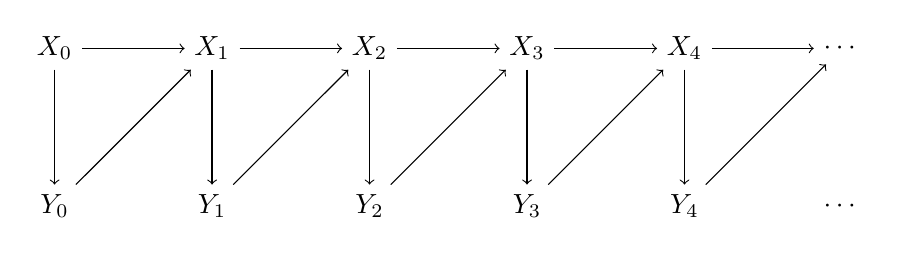
\begin{tikzpicture}[xscale=2,yscale=1]
  \node (x0) at (0,2){$X_0$};
  \node (x1) at (1,2){$X_1$};
  \node (x2) at (2,2){$X_2$};
  \node (x3) at (3,2){$X_3$};
  \node (x4) at (4,2){$X_4$};
  \node (x5) at (5,2){$\cdots$};

  \node (y0) at (0,0){$Y_0$};
  \node (y1) at (1,0){$Y_1$};
  \node (y2) at (2,0){$Y_2$};
  \node (y3) at (3,0){$Y_3$};
  \node (y4) at (4,0){$Y_4$};
  \node (y5) at (5,0){$\cdots$};

  \draw[->] (x0) -- (x1);
  \draw[->] (x1) -- (x2);
  \draw[->] (x2) -- (x3);
  \draw[->] (x3) -- (x4);
  \draw[->] (x4) -- (x5);

  \draw[->] (x0) -- (y0);
	\draw[->] (x1) -- (y1);
	\draw[->] (x2) -- (y2);
	\draw[->] (x3) -- (y3);
	\draw[->] (x4) -- (y4);

  \draw[->] (y0) -- (x1);
  \draw[->] (y1) -- (x2);
  \draw[->] (y2) -- (x3);
  \draw[->] (y3) -- (x4);
  \draw[->] (y4) -- (x5);

\end{tikzpicture}
\caption{The Dependencies between $X_t$ and $Y_t$}
\label{Mardep}
\end{figure}
Their dependency relationships are visualized in Figure~\ref{Mardep}. We can see that $X_t$ depends directly on $X_{t-1}$ and $Y_{t-1}$, whereas $Y_t$ only depends directly on $X_t$.  

This again corresponds to the next board-state only depending directly on the current world-state and the current move, which in turn only depends on the current board-state, which directly corresponds to our intuition of how a Tic-Tac-Toe game works. 

%\subsection{Modeling the System using a MDP and a Policy}
\subsection{Markov Decision Procedures and a Policy}
To begin our definition of the MDP, we define {\bf{Markov Matrices}} $M^{a_j}\in \mathbb{R}^{n \times n}$ with 
\[
M^{a_j}_{x,y}:=P(X_{t+1}=q_x|X_{t=q_y},Y_t=a_j)
\]
We observe that these probabilities are invariant under $t$.  

In our running example of a Tic-Tac-Toe game, these matrices would consist of mainly $0$s and $1$s, however, for most situations commonly modeled by MDPs, the entries of $M^{a_j}$ only need to satisfy the condition that $M^{a_j}$ has column sums of $1$ and non-negative entries. 

To choose actions, we define a map $\pi:Q\rightarrow \mathbb{R}^{m}$, which we call the {\bf{policy}}, with $\pi(q_i)[j]=P(Y_t=a_j|X_t=q_i)$. Hence we require that for all $q_i$ in $Q$
\[
\sum\limits_{j=1}^{m} \pi(q_i)[j] =1 
\]
We write $v[j]$ for the $j$-th entry of any vector $v$.
A policy for our Tic-Tac-Toe game could, for example, be always placing an {\ticX} in the middle when possible and else randomly placing the {\ticX} on a free position. 

We now want to be able to predict the future and compute probabilities for a realization of this process with a history of world-states and actions $X_0=q_{i_0},Y_0={a_{j_0}},\ldots,X_{t-1}=q_{i_{t-1}},Y_{t-1}=a_{j_{t-1}}$. We write $q_{i_0},a_{j_0},\ldots,q_{i_{t-1}},a_{j_{t-1}}$ as shorthand for this history of world-states and actions. To save space we also often write $h$ to refer to this history.
 
We define a vector $w_t\in \mathbb{R}^{n}$ containing the probabilities of the world at time $t$ being in state $q_i$ for a given realization of the process up to time $t-1$ by
\[
w_t:=
\left (
\begin{matrix}
P(X_t=q_1|q_{i_0},a_{j_0},\ldots,q_{i_{t-1}},a_{j_{t-1}}) \\
P(X_t=q_2|q_{i_0},a_{j_0},\ldots,q_{i_{t-1}},a_{j_{t-1}}) \\
\vdots \\
P(X_t=q_n|q_{i_0},a_{j_0},\ldots,q_{i_{t-1}},a_{j_{t-1}})
\end{matrix}
\right )
=
\left (
\begin{matrix}
P(X_t=q_1|q_{i_{t-1}},a_{j_{t-1}}) \\
P(X_t=q_2|q_{i_{t-1}},a_{j_{t-1}}) \\
\vdots \\
P(X_t=q_n|q_{i_{t-1}},a_{j_{t-1}})
\end{matrix}
\right )
\]
We note that this is equal to the $i_{t-1}$th column of $M^{a_{j_{t-1}}}$, hence we can compute $w_t=M^{a_{j_{t-1}}}*e_{i_{t-1}}$, where $e_i$ is the standard basis vector of $\mathbb{R}^{n}$ containing only zeroes, except for 1 in the $i$-th entry. 

Similarly, we define vectors $w_t^{t+k} \in \mathbb{R}^{n}$ with $k\in \mathbb{N}$ and
\[
w_t^{t+k}:=
\left (
\begin{matrix}
P(X_{t+k}=q_1|q_{i_0},a_{j_0},\ldots,q_{i_{t-1}},a_{j_{t-1}}) \\
P(X_{t+k}=q_2|q_{i_0},a_{j_0},\ldots,q_{i_{t-1}},a_{j_{t-1}}) \\
\vdots \\
P(X_{t+k}=q_n|q_{i_0},a_{j_0},\ldots,q_{i_{t-1}},a_{j_{t-1}})
\end{matrix}
\right)
=
\left (
\begin{matrix}
P(X_{t+k}=q_1|q_{i_{t-1}},a_{j_{t-1}}) \\
P(X_{t+k}=q_2|q_{i_{t-1}},a_{j_{t-1}}) \\
\vdots \\
P(X_{t+k}=q_n|q_{i_{t-1}},a_{j_{t-1}})
\end{matrix}
\right )
\]
Since we can easily compute $P(Y_{t+k}=a_j|X_{t+k}=q_i)$ using $\pi(q_i)$, our goal of being able to predict the future is equivalent to being able to compute $w_t^{t+k}$.
\begin{prop}
We can compute $w_t^{t+k+1}[i]$ by $\sum\limits_{d=1}^{n} w_t^{t+k}[d] \sum\limits_{j=1}^{m} M^{a_j}_{i,d} \cdot \pi(q_d)[j]$.
\end{prop}
\begin{proof}
We compute directly
\begin{align*}
&w_t^{t+k+1}[i]\\
=&P(X_{t+k+1}=q_i|q_{i_0},a_{j_0},\ldots,q_{i_{t-1}},a_{j_{t-1}}) \\
=&P(X_{t+k+1}=q_i|q_{i_{t-1}},a_{j_{t-1}}) \\
=&\sum\limits_{j=1}^{m} \sum\limits_{d=1}^{n} P(X_{t+k+1}=q_i,X_{t+k}=q_d,Y_{t+k}=a_j|q_{i_{t-1}},a_{j_{t-1}}) \\
=&\sum\limits_{j=1}^{m} \sum\limits_{d=1}^{n} P(X_{t+k+1}=q_i,X_{t+k}=q_d|Y_{t+k}=a_j,q_{i_{t-1}},a_{j_{t_1}})\cdot P(Y_{t+k-1}=a_j|q_{i_{t-1}},a_{j_{t-1}}) \\
=&\sum\limits_{j=1}^{m} \sum\limits_{d=1}^{n} P(X_{t+k+1}=q_i|X_{t+k}=q_d,Y_{t+k}=a_j,h)\cdot P(X_{t+k}=q_d|Y_{t+k}=a_j,h)\cdot P(Y_{t+k}=a_j|h) \\
=&\sum\limits_{j=1}^{m} \sum\limits_{d=1}^{n} P(X_{t+k+1}=q_i|X_{t+k}=q_d,Y_{t+k}=a_j)\cdot P(X_{t+k}=q_d|Y_{t+k}=a_j,h)\cdot P(Y_{t+k}=a_j|h) \\
=&\sum\limits_{j=1}^{m} \sum\limits_{d=1}^{n}  P(X_{t+k+1}=q_i|X_{t+k}=q_d,Y_{t+k}=a_j)\cdot P(Y_{t+k}=a_j|X_{t+k}=q_d,h)\\
   & \phantom{\sum\limits_{j=1}^{m} \sum\limits_{d=1}^{n}}\cdot \frac{P(X_{t+k}=q_d|h)}{P(Y_{t+k}=a_j|h)} \cdot P(Y_{t+k}=a_j|h)\\
=&\sum\limits_{j=1}^{m} \sum\limits_{d=1}^{n} P(X_{t+k+1}=q_i|X_{t+k}=q_d,Y_{t+k}=a_j)\cdot P(Y_{t+k}=a_j|X_{t+k}=q_d,h)\cdot P(X_{t+k}=q_d|h) \\
=&\sum\limits_{j=1}^{m} \sum\limits_{d=1}^{n} M^{a_j}_{i,d} \cdot \pi(q_d)[j]\cdot w_t^{t+k}[d] \\
=&\sum\limits_{d=1}^{n} w_t^{t+k}[d] \sum\limits_{j=1}^{m} M^{a_j}_{i,d} \cdot \pi(q_d)[j]
\end{align*}
\end{proof}
Then as a direct corollary we can write $w_t^{t+k+1}$ as 
\[
w_t^{t+k+1}=\sum\limits_{d=1}^{n} w_t^{t+k}[d] \sum\limits_{j=1}^{m} M^{a_j}*e_d\cdot \pi(q_d)[j]
\]
Hence we can compute $w_t^{t+k+1}$ in terms of $w_t^{t+k}$. Therefore we can iteratively compute $w_t^{t+k+1}$, where every step is computable in $O(m*n^3)$, using normal matrix multiplication. 

Thus, we have fulfilled one part of the MC goal, as we have found a way to predict the future in $k$ steps in a fashion that is linear in $k$, and hence can feasibly be computed. 

%\subsection{Modeling the System with a MC}
\subsection{Markov Chains}
Now we will try to fulfill the other part of the {\mc} goal, by defining a MC, that models the same process. Since we are building a MC from a MDP and a policy, this means that we aren't going to be fulfilling the goal entirely. Not every MC has an equivalent MDP and a policy, but at least a subset of them can be represented using a MDP and a policy. We can actually define two MCs that model the same process, once as a plain MC with world-states $Q$ and once as a MC with world-states from $Q\times A$. 

To specify the first option, we first define its Markov matrix $M \in \mathbb{R}^{n\times n}$: 
\[
M:=
\left (
\begin{matrix}
P(X_{t+1}=q_1|X_{t}=q_1) &  \ldots & P(X_{t+1}=q_1|X_t=q_n) \\
\vdots & \vdots & \vdots \\
P(X_{t+1}=q_n|X_t=q_1) & \ldots & P(X_{t+1}=q_n|X_t=q_n) 
\end{matrix}
\right )
\]
\begin{prop}
We can compute the entries of $M$ using $M^{a_j}$ and $\pi$ by $M_{x,y}=\sum\limits_{j=1}^{m} M^{a_j}_{x,y}*\pi(y)[j]$.
\end{prop} 
\begin{proof}
\begin{align*}
M_{i_1,i_2}&=\sum\limits_{j=1}^{m} \pi(q_{i_2})[j]M^{a_j}_{i_1,i_2} \\
&=\sum\limits_{j=1}^{m} P(Y_{t}=a_j|X_t=q_{i_2})\cdot P(X_{t+1}=q_{i_1}|X_t=q_{i_2},Y_t=a_j) \\
&=\sum\limits_{j=1}^{m} P(Y_t=a_j,X_{t+1}=q_{i_1}|X_t=q_{i_2}) \\
&=P(X_{t+1}=q_{i_1}|X_t=q_{i_2})
\end{align*}
\end{proof}
\begin{prop}
We can use $M$ to compute $w_t^{t+k+1}[i]=(M*w_t^{t+k})[i]$.
\end{prop}
\begin{proof}
\begin{align*}
w_t^{t+k+1}[i]&=P(X_{t+k+1}=q_i|q_{i_0},a_{j_0},\ldots,q_{i_{t-1}},a_{j_{t-1}}) \\
&=\sum\limits_{d=1}^{n} P(X_{t+k+1}=q_i,X_{t+k}=q_d|q_{i_0},a_{j_0},\ldots,q_{i_{t-1}},a_{j_{t-1}}) \\
&=\sum\limits_{d=1}^{n} P(X_{t+k+1}=q_i|X_{t+k}=q_d,q_{i_0},a_{j_0},\ldots,q_{i_{t-1}},a_{j_{t-1}})\cdot \\
& \phantom{= \sum\limits_{d=1}^{n}} P(X_{t+k}=q_d|q_{i_0},a_{j_0},\ldots,q_{i_{t-1}},a_{j_{t-1}}) \\
&=\sum\limits_{d=1}^{n} P(X_{t+k+1}=q_i|X_{t+k}=q_d)\cdot P(X_{t+k}=q_d|q_{i_0},a_{j_0},\ldots,q_{i_{t-1}},a_{j_{t-1}}) \\
&=(M*w_t^{t+k})[i]
\end{align*}
\end{proof}
Hence we get 
\[
w_t^{t+k+1}=M*w_t^{t+k}
\]
We note that using this method, every step is in $O(n^3)$ and therefore represents an even faster way of computing $w_t^{t+k}$. However, it does not quite replicate the structure of our previous model, as we can't look at different actions and their consequences anymore.

We can additionally model the entire process using a MC with world-states $(q_i,a_j) \in Q \times A$. The corresponding Markov matrix $\widetilde{M}$ is given by 
%This is where the label used to be, when stuff didn't work correctly. Just for documentation purpoes.
\label{MC:HMM2}
{\footnotesize
\[\setlength{\arraycolsep}{0pt} 
\widetilde{M}:=
\left ( 
\begin{matrix}
\pi(q_1)[1]\cdot (M^{a_1})_{1,1} & \pi(q_1)[1]\cdot (M^{a_2})_{1,1} & \ldots & \pi(q_1)[1]\cdot (M^{a_m})_{1,1} & \pi(q_1)[1]\cdot (M^{a_1})_{1,2} & \ldots & \pi(q_1)[1]\cdot (M^{a_m})_{1,n} \\
\pi(q_1)[2]\cdot (M^{a_1})_{1,1} & \pi(q_1)[2]\cdot (M^{a_2})_{1,1} & \ldots & \pi(q_1)[2]\cdot (M^{a_m})_{1,1} & \pi(q_1)[2]\cdot (M^{a_1})_{1,2} & \ldots &\pi(q_1)[2]\cdot (M^{a_m})_{1,n} \\
\vdots \\
\pi(q_1)[m]\cdot (M^{a_1})_{1,1} & \pi(q_1)[m]\cdot (M^{a_2})_{1,1} & \ldots & \pi(q_1)[m]\cdot (M^{a_m})_{1,1} & \pi(q_1)[m]\cdot (M^{a_1})_{1,2} & \ldots & \pi(q_1)[m]\cdot (M^{a_m})_{1,n} \\
\pi(q_2)[1]\cdot (M^{a_1})_{2,1} & \pi(q_2)[1]\cdot (M^{a_2})_{2,1} & \ldots & \pi(q_2)[1]\cdot (M^{a_m})_{2,1} & \pi(q_2)[1]\cdot (M^{a_1})_{2,2} & \ldots & \pi(q_2)[1]\cdot (M^{a_m})_{2,n} \\
\vdots \\ 
\pi(q_n)[m]\cdot (M^{a_1})_{n,1} & \pi(q_n)[m]\cdot (M^{a_2})_{n,1} & \ldots & \pi(q_n)[m]\cdot (M^{a_m})_{n,1} & \pi(q_n)[m]\cdot (M^{a_1})_{n,2} & \ldots & \pi(q_n)[m]\cdot (M^{a_m})_{n,n} \\
\end{matrix} 
\right )
\]
}
\begin{prop}
$\widetilde{M}$ has as entries the probabilities $\widetilde{M}_{(i_1-1) \cdot m+j_1,(i_2-1) \cdot m+j_2}=P(X_{t+1}=q_{i_1},Y_{t+1}=a_{j_1}|X_{t}=q_{i_2},Y_t=a_{j_2})$.
\end{prop}
\begin{proof}
\begin{align*}
\widetilde{M}_{(i_1-1)\cdot m+j_1,(i_2-1)\cdot m+j_2}&=\pi(q_{i_1})[j_1]\cdot M^{a_{j_2}}_{i_1,i_2}  \\
&=P(Y_{t}=a_{j_1}|X_{t}=q_{i_1})\cdot P(X_t=q_{i_1}|X_{t-1}=q_{i_2},Y_{t-1}=a_{j_1}) \\
&=P(Y_{t}=a_{j_1}|X_t=q_{i_1},Y_{t-1}=a_{j_1})\cdot P(X_t=q_{i_1}|X_{t-1}=q_{i_2},Y_{t-1}=a_{j_1}) \\
&=P(Y_{t}=a_{j_1},X_t=q_{i_1}|Y_{t-1}=a_{j_1},X_{t-1}=q_{i_2})
\end{align*}
\end{proof}
Since our process now has a higher dimension, we need to define higher dimensional $\widetilde{w_t}\in \mathbb{R}^{nm}$ by
\[
\widetilde{w_t}:=\left ( 
\begin{matrix} 
P(X_t=q_1,Y_t=a_1|q_{i_0},a_{j_0},\ldots,q_{i_{t-1}},a_{j_{t-1}}) \\
P(X_t=q_1,Y_t=a_2|q_{i_0},a_{j_0}\ldots,q_{i_{t-1}},a_{j_{t-1}}) \\
\vdots \\
P(X_t=q_1,Y_t=a_m|q_{i_0},a_{j_0}\ldots,q_{i_{t-1}},a_{j_{t-1}}) \\
P(X_t=q_2,Y_t=a_1|q_{i_0},a_{j_0}\ldots,q_{i_{t-1}},a_{j_{t-1}}) \\ 
\vdots \\
P(X_t=q_n,Y_t=a_m|q_{i_0},a_{j_0}\ldots,q_{i_{t-1}},a_{j_{t-1}})
\end{matrix} 
\right )
\]
In contrast to $w_t$ every entry now contains the probability of action $a_j$ and world-state $q_i$, instead of just the probability of $q_i$. We can easily compute $\widetilde{w_t}$ from $w_t$ by $\widetilde{w_t}[(i-1) \cdot m+j]=\pi(q_i)[j]\cdot w_t[i]$.
Similarly, we define $\widetilde{w_t}^{t+k}$ as 
\[
\widetilde{w_t}^{t+k}:=
\left ( 
\begin{matrix}
P(X_{t+k}=q_1,Y_{t+k}=a_1|q_{i_0},a_{j_0},\ldots,q_{i_{t-1}},a_{j_{t-1}}) \\
P(X_{t+k}=q_1,Y_{t+k}=a_2|q_{i_0},a_{j_0},\ldots,q_{i_{t-1}},a_{j_{t-1}}) \\
\vdots \\
P(X_{t+k}=q_n,Y_{t+k}=a_m|q_{i_0},a_{j_0},\ldots,q_{i_{t-1}},a_{j_{t-1}}) \\
\end{matrix}
\right )
\]
\begin{prop} We can compute $\widetilde{w_t}^{t+k+1}=\widetilde{M}*\widetilde{w_t}^{t+k}$.
\end{prop}
\begin{proof}
\begin{align*}
&w_t^{t+k+1}[(i-1)\cdot m+j] \\&=P(X_{t+k}=q_1,Y_{t+k}=a_1|q_{i_0},a_{j_0},\ldots,q_{i_{t-1}},a_{j_{t-1}}) \\
&=\sum\limits_{j_1=1}^{m} \sum\limits_{i_1=1}^{n} P(X_{t+k+1}=q_i,Y_{t+k+1}=a_j,X_{t+k}=q_{i_1},Y_{t+k}=a_{j_1}|q_{i_0},a_{j_0},\ldots,q_{i_{t-1}},a_{j_{t-1}})\\
&=\sum\limits_{j_1=1}^{m} \sum\limits_{i_1=1}^{n} P(X_{t+k+1}=q_i,Y_{t+k+1}=a_j,X_{t+k}=q_{i_1},Y_{t+k}=a_{j_1}|h) \\
&=\sum\limits_{j_1=1}^{m} \sum\limits_{i_1=1}^{n} P(X_{t+k+1}=q_i,Y_{t+k+1}=a_j|X_{t+k}=q_{i_1},Y_{t+k}=a_{j_1},h)\cdot P(X_{t+k}=q_{i_1},Y_{t+k}=a_{j_1}|h) \\
&=(M*w_t^{t+k})[(i-1) \cdot m+j]
\end{align*}
\end{proof}
This means that we can also predict the future using this model, which has world-states of $Q\times A$, and therefore is in the form described in Dragan's paper. Since we have shown that this describes the same process as our formulation with a MDP and a policy, we have fulfilled the first part of the MC goal. 

\bigskip
Now that we have fulfilled both parts of the our first goal, we move onto the more ambitious HMM goal.
\section{The Hidden Markov Model Case:  Evaluating the Coverage of the EPA}\label{sec:HMM}
By looking at HMMs we can cover a broader range of stochastic processes, because we can account for hidden variables that are not immediately obvious, hence results on whether HMMs/POMDPs can be covered show how broad the coverage of the EPA is.
\subsection{System Definition}
The main difference between the assumptions of a Markov Decision Process and those of a \emph{Partially Observable} Markov Decision Process is, that the agent cannot directly perceive the world-states $q_i$ anymore. Instead, it can only observe from a set $O=\{o_1,\ldots,o_K\}$ of observables, which are emitted with fixed probabilities depending on the world-states. It is then possible to estimate the world-states based on the observed history of observables and actions. 

For our running example of a Tic-Tac-Toe game, this could translate to taking off one's glasses while playing the game. Then it might be possible to observe an {\ticO}, where there should be an {\ticX}. Thus, we could get observations $O$ like:
\[
O=\{
\left ( 
\begin{matrix}
e & e & e \\
e & e & e \\
e & e & e \\ 
\end{matrix}
\right )
,
\left ( 
\begin{matrix}
{\ticX} & e & e \\
e & e & e \\
e & e & e \\ 
\end{matrix}
\right )
,
\left ( 
\begin{matrix}
{\ticX} & {\ticX} & e \\
e & e & e \\
e & e & e \\ 
\end{matrix}
\right ), \ldots,
\left ( 
\begin{matrix}
{\ticX} & {\ticX} & {\ticX} \\
{\ticX} & {\ticX} & {\ticX} \\
{\ticX} & {\ticX} & {\ticX} \\ 
\end{matrix}
\right )
\]
We notice that this includes game states which would be impossible to observe in an actual game. This is because the set of observables $O$ is in most cases substantially different from the set of world-states $Q$. 

Similarly to before we describe actions, observables, and world-states using random variables. We again use $X_t$ and $Y_t$ for world-states and actions at time $t$ respectively, but additionally add $Z_t:\Omega \rightarrow O$ for the observables. 
\begin{figure}\centering
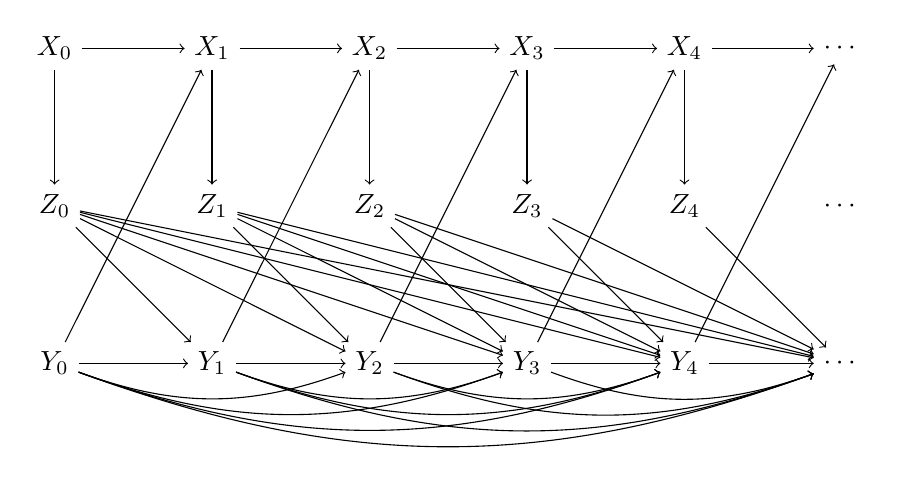
\begin{tikzpicture}[xscale=2,yscale=2]
  \node (x0) at (0,2){$X_0$};
  \node (x1) at (1,2){$X_1$};
  \node (x2) at (2,2){$X_2$};
  \node (x3) at (3,2){$X_3$};
  \node (x4) at (4,2){$X_4$};
  \node (x5) at (5,2){$\cdots$};

  \node (z0) at (0,1){$Z_0$};
  \node (z1) at (1,1){$Z_1$};
  \node (z2) at (2,1){$Z_2$};
  \node (z3) at (3,1){$Z_3$};
  \node (z4) at (4,1){$Z_4$};
  \node (z5) at (5,1){$\cdots$};

  \node (y0) at (0,0){$Y_0$};
  \node (y1) at (1,0){$Y_1$};
  \node (y2) at (2,0){$Y_2$};
  \node (y3) at (3,0){$Y_3$};
  \node (y4) at (4,0){$Y_4$};
  \node (y5) at (5,0){$\cdots$};

  \draw[->] (x0) -- (x1);
  \draw[->] (x1) -- (x2);
  \draw[->] (x2) -- (x3);
  \draw[->] (x3) -- (x4);
  \draw[->] (x4) -- (x5);

  \draw[->] (x0) -- (z0);
  \draw[->] (x1) -- (z1);
  \draw[->] (x2) -- (z2);
  \draw[->] (x3) -- (z3);
  \draw[->] (x4) -- (z4);


  \draw[->] (y0) -- (x1);
  \draw[->] (y1) -- (x2);
  \draw[->] (y2) -- (x3);
  \draw[->] (y3) -- (x4);
  \draw[->] (y4) -- (x5);

  \draw[->] (y0) -- (y1);
  \draw[->] (y0) to[bend right=20] (y2);
  \draw[->] (y0) to[bend right=20] (y3);
  \draw[->] (y0) to[bend right=20] (y4);
  \draw[->] (y0) to[bend right=20] (y5);
	
	\draw[->] (y1) -- (y2);
  \draw[->] (y1) to[bend right=20] (y3);
  \draw[->] (y1) to[bend right=20] (y4);
  \draw[->] (y1) to[bend right=20] (y5);
 
	
	\draw[->] (y2) -- (y3);
  \draw[->] (y2) to[bend right=20] (y4);
  \draw[->] (y2) to[bend right=20] (y5);

  \draw[->] (y3) -- (y4);
  \draw[->] (y3) to[bend right=20] (y5);

	\draw[->] (y4) to (y5);

  \draw[->] (z0) -- (y1);
  \draw[->] (z0) -- (y2);
  \draw[->] (z0) -- (y3);
  \draw[->] (z0) -- (y4);
  \draw[->] (z0) -- (y5);

  \draw[->] (z1) -- (y2);
  \draw[->] (z1) -- (y3);
  \draw[->] (z1) -- (y4);
  \draw[->] (z1) -- (y5);

  \draw[->] (z2) -- (y3);
  \draw[->] (z2) -- (y4);
  \draw[->] (z2) -- (y5);

  \draw[->] (z3) -- (y4);
  \draw[->] (z3) -- (y5);

  \draw[->] (z4) -- (y5);
\end{tikzpicture}
\caption{The Relationships between $X_t$, $Y_t$ and $Z_t$}
\label{HMMdep}
\end{figure}
We can see their inter-dependencies in Figure~\ref{HMMdep}. We notice that the $X_t$ remain unchanged, they only depends directly on $X_{t-1}$ and $Y_{t-1}$. Then we have an added row of $Z_t$, which depend directly on $X_t$. The largest divergence to the previous case is in the choice of actions. $Y_t$ does not depend directly on $X_t$ anymore instead depending on all previous observables and actions. This is because the agent has no way of knowing what the current world-state is and has to infer it based on its previous perceived history. 

One direct consequence is that $P(X_t=q_i|a_{j_0},o_{e_0},\ldots,a_{j_{t-1}},O_{e_{t-1}})$ is independent of $P(Y_t=a_j|h)$ for all $q_i\in Q$ and $a_j\in A$, given a history of actions and observables. Hence we have that $P(Y_t=a_j|X_t=q_{i_1},h)=P(Y_t=a_j|X_t=q_{i_2},h) \qquad \forall q_{i_1},q_{i_2} \in Q$. 
We note that $h$ here has a slightly different meaning than before, as it is now a history of observables and actions, not a history of actions and world-states. 

%\subsection{Modeling the System using a POMDP and a Policy}
\subsection{Partially Observable Markov Decision Procedures and a Policy}
We again define a vector $w_t\in \mathbb{R}^{n}$ containing the probability that at time $t$ the world is in world-state $q_i$ given a previous history as 
\[
w_t:=
\left ( 
\begin{matrix}
P(X_t=q_1|o_{e_0},a_{j_0},\ldots,o_{e_{t-1}},a_{j_{t-1}}) \\
P(X_t=q_2|o_{e_0},a_{j_0},\ldots,o_{e_{t-1}},a_{j_{t-1}}) \\
\vdots \\
P(X_t=q_n|o_{e_0},a_{j_0},\ldots,o_{e_{t-1}},a_{j_{t-1}}) 
\end{matrix}
\right )
\]
One important difference to our definition of $w_t$ in the {\mc} case is that $P(X_t=q_i|o_{e_0},a_{j_0},\ldots,o_{e_{t-1}},a_{j_{t-1}})$ is not necessarily equal to $P(X_t=q_n|q_{i_{t-1}},a_{j_{t-1}})$. Here, we really need the full history for our definition. 

We again define $w_t^{t+k}$ as 
\[
w_t^{t+k}:=
\left ( 
\begin{matrix}
P(X_{t+k}=q_1|o_{e_0},a_{j_0},\ldots,o_{e_{t-1}},a_{j_{t-1}}) \\
P(X_{t+k}=q_2|o_{e_0},a_{j_0},\ldots,o_{e_{t-1}},a_{j_{t-1}}) \\
\vdots \\
P(X_{t+k}=q_n|o_{e_0},a_{j_0},\ldots,o_{e_{t-1}},a_{j_{t-1}}) 
\end{matrix}
\right )
\]
As before, we will try to compute $w_t^{t+k}$ to fulfill the second part of the HMM goal. 
We define Markov matrices $M^{a_j}$ with entries 
\[
M^{a_j}_{x,y}:=P(X_{t+1}=q_x|X_{t}=q_y,Y_t=a_j)=P(X_{t+1}=q_x|X_t=q_y,Y_t=a_j,h)
\]
as we have done for the {\mc} case in Section~\ref{sec:MC}.  To deal with the added
observables we define a $n\times n$ diagonal observation matrices $O_{o_e}$ with diagonal
entries containing the probability of observing $o_e$, given the current world-state:
\[
(O_{o_e})_{i,i}:=P(Z_t=o_e|X_t=q_i)=P(Z_t=o_e|X_t=q_i,Y_t=a_j)
\]
We note that the observation probability is independent of the action, as indicated in Figure $\ref{HMMdep}$. 
Then we also define operators $T^{a_j}_{o_e}=M^{a_j}*O_{o_e}$. 
\begin{prop}
$(T^{a_j}_{o_e})_{x,y}=P(X_{t+1}=q_x,Z_t=o_e|Y_t=a_j,X_t=q_y)$ 
\end{prop}
\begin{proof}
\begin{align*}
(T^{a_j}_{o_e})_{x,y}&=(M^{a_j}*O_{o_e})_{x,y} \\
&=\sum\limits_{d=1}^{n} M^{a_j}_{x,d}\cdot (O_{o_e})_{d,y} \\
&=M^{a_j}_{x,y}\cdot (O_{o_e})_{y,y} \\
&=P(X_{t+1}=q_x|Y_t=a_j,X_t=q_y)\cdot P(Z_t=o_e|X_t=q_y) \\
&=P(X_{t+1}=q_x|Y_t=a_j,X_t=q_y)\cdot P(Z_t=o_e|X_t=q_y,Y_t=a_j) \\
&=P(X_{t+1}=q_x,Z_t=o_e|Y_t=a_j,X_t=q_y)
\end{align*}
\end{proof}
This is not something conventionally used for computations in HMMs/POMDPs. However, we use it because it is very similar to OOMs and we are looking at HMMs/POMDPs as a special case of OOMs/IO-OOMs, since OOMs were the original tool used by Dragan. 

We can now use these operators to compute the probability of observing $o_e$ given an action $a_j$ and a history $h$. 
\begin{prop}
$P(Z_t=o_e|Y_t=a_j,h)=\vec{1}*T^{a_j}_{o_e}*w_t$ 
\end{prop}
\begin{proof}
We prove this by inserting definitions and computing. The major trick we use is that $P(Y_t=a_j|h)=P(Y_t=a_j|X_t=q_i,h)$.
\begin{align*}
\vec{1}*T^{a_j}_{o_e}*w_t&=\sum\limits_{i=1}^{n} (T^{a_j}_{o_e})_{i,:}*w_t \\
&=\sum\limits_{i=1}^{n} \sum\limits_{d=1}^{n} P(X_{t+1}=q_i,Z_t=o_e|X_t=q_d,Y_t=a_j)\cdot P(X_t=q_d|h) \\
&=\sum\limits_{i=1}^{n} \sum\limits_{d=1}^{n} P(X_{t+1}=q_i,Z_t=o_e|X_t=q_d,Y_t=a_j)\cdot P(X_t=q_d|h)\cdot \frac{P(Y_t=a_j|h)}{P(Y_t=a_j|h)} \\
&=\frac{\sum\limits_{i=1}^{n} \sum\limits_{d=1}^{n} P(X_{t+1}=q_i,Z_t=o_e|X_t=q_d,Y_t=a_j)\cdot P(X_t=q_d|h)\cdot P(Y_t=a_j|h)}{P(Y_t=a_j|h)} \\
&=\frac{\sum\limits_{i=1}^{n} \sum\limits_{d=1}^{n} P(X_{t+1}=q_i,Z_t=o_e|X_t=q_d,Y_t=a_j)\cdot P(X_t=q_d|h)\cdot P(Y_t=a_j|X_t=q_d,h)}{P(Y_t=a_j|h)} \\
&=\frac{\sum\limits_{i=1}^{n} \sum\limits_{d=1}^{n} P(X_{t+1}=q_i,Z_t=o_e|X_t=q_d,Y_t=a_j)\cdot P(X_t=q_d,Y_t=a_j|h)}{P(Y_t=a_j|h)} \\
&=\frac{\sum\limits_{i=1}^{n} \sum\limits_{d=1}^{n} P(X_{t+1}=q_i,Z_t=o_e|X_t=q_d,Y_t=a_j,h)\cdot P(X_t=q_d,Y_t=a_j|h)}{P(Y_t=a_j|h)} \\
&=\frac{\sum\limits_{i=1}^{n} \sum\limits_{d=1}^{n} P(X_{t+1}=q_i,Z_t=o_e,X_t=q_d,Y_t=a_j|h)}{P(Y_t=a_j|h)} \\
&=\frac{ P(Z_t=o_e,Y_t=a_j|h)}{P(Y_t=a_j|h)} \\
&=P(Z_t=o_e|Y_t=a_j,h)
\end{align*}
Here we wrote $(T^{a_j}_{o_e})_{i,:}$ for the $i$-th row of $T^{a_j}_{o_e}$. 
\end{proof}
We can even simplify this further by noting that $M^{a_j}$ has column sums equal to $1$, hence $\vec{1}M^{a_j}*v=\vec{1}*v$ for all vectors $v$ in $\mathbb{R}^n$, hence 
\[
P(Z_t=o_e|Y_t=a_j,h)=\vec{1}T^{a_j}_{o_e}*w_t=\vec{1}M^{a_j}*O_{o_e}*w_t=\vec{1}O_{o_e}*w_t=P(Z_t=o_e|Y_t=a_{j_1},h)
\]
from which we conclude that $P(Z_t=o_e|h)=\vec{1}O_{o_e}*w_t$. 

Using a similar trick we can compute $P(X_{t+1}=q_i|Z_t=o_e,Y_t=a_j,h)$ by computing $(T^{a_j}_{o_e}*w_t)[i]$ and then normalizing it.
\begin{prop}
$P(X_{t+1}=q_i|Z_t=o_e,Y_t=a_j,h)=(\frac{T^{a_j}_{o_e}*w_t}{\vec{1}T^{a_j}_{o_e}*w_t})[i]$
\end{prop}
\begin{proof}
\begin{align*}
(\frac{T^{a_j}_{o_e}*w_t}{\vec{1}T^{a_j}_{o_e}*w_t})[i]&=\frac{\sum\limits_{d=1}^{n} (T^{a_j}_{o_e})_{i,d}\cdot w_t[d]}{\sum\limits_{i=1}^n\sum\limits_{d=1}^{n} (T^{a_j}_{o_e})_{i,d}\cdot w_t[d]} \\
&=\frac{\sum\limits_{d=1}^{n} P(Z_t=o_e,X_{t+1}=q_i|Y_t=a_j,X_t=q_d)\cdot P(X_t=q_d|h)}{\sum\limits_{i=1}^n\sum\limits_{d=1}^{n} P(Z_t=o_e,X_{t+1}=q_i|Y_t=a_j,X_t=q_d)\cdot P(X_t=q_d|h)} \\
&=\frac{\sum\limits_{d=1}^{n} P(Z_t=o_e,X_{t+1}=q_i|Y_t=a_j,X_t=q_d)\cdot P(X_t=q_d|h)}{\sum\limits_{i=1}^n\sum\limits_{d=1}^{n} P(Z_t=o_e,X_{t+1}=q_i|Y_t=a_j,X_t=q_d)\cdot P(X_t=q_d|h)}\cdot \frac{P(Y_t=a_j|h)}{P(Y_t=a_j|h)} \\
&=\frac{\sum\limits_{d=1}^{n} P(Z_t=o_e,X_{t+1}=q_i|Y_t=a_j,X_t=q_d)\cdot P(X_t=q_d|h)\cdot P(Y_t=a_j|h)}{\sum\limits_{i=1}^n\sum\limits_{d=1}^{n} P(Z_t=o_e,X_{t+1}=q_i|Y_t=a_j,X_t=q_d)\cdot P(X_t=q_d|h)\cdot P(Y_t=a_j|h)} \\
&=\frac{\sum\limits_{d=1}^{n} P(Z_t=o_e,X_{t+1}=q_i|Y_t=a_j,X_t=q_d)\cdot P(Y_t=a_j,X_t=q_d|h)}{\sum\limits_{i=1}^n\sum\limits_{d=1}^{n} P(Z_t=o_e,X_{t+1}=q_i|Y_t=a_j,X_t=q_d)\cdot P(Y_t=a_j,X_t=q_d|h)} \\
&=\frac{\sum\limits_{d=1}^{n} P(Z_t=o_e,X_{t+1}=q_i|Y_t=a_j,X_t=q_d,h)\cdot P(Y_t=a_j,X_t=q_d|h)}{\sum\limits_{i=1}^n\sum\limits_{d=1}^{n} P(Z_t=o_e,X_{t+1}=q_i|Y_t=a_j,X_t=q_d,h)\cdot P(Y_t=a_j,X_t=q_d|h)} \\
&=\frac{\sum\limits_{d=1}^{n} P(Z_t=o_e,X_{t+1}=q_i,Y_t=a_j,X_t=q_d|h)}{\sum\limits_{i=1}^{n} \sum\limits_{d=1}^{n} P(Z_t=o_e,X_{t+1}=q_i,Y_t=a_j,X_t=q_d|h)|} \\
&=\frac{P(Z_t=o_e,X_{t+1}=q_i,Y_t=a_j|h)}{P(Z_t=o_e,Y_t=a_j|h)} \\
&=P(X_{t+1}=q_i|Z_t=o_e,Y_t=a_j,h)
\end{align*}
\end{proof}
We use this result to compute $w_t$. We start out with the initial distribution $w_0$ such that $w_0[i]=P(X_0=q_i)$. When we observe $o_{e_0}$ and take $a_{j_0}$, we update to $w_1=\frac{T^{a_{j_0}}_{o_{e_0}}*w_0}{\vec{1}*T^{a_{j_0}}_{o_{e_0}}*w_0}$ and so on. For this reason, we refer to this equation as an {\textbf{update equation}}. 

However, all of these probabilities so far have been contingent on the choice of action. As a consequence we also need to define a way to choose actions. 
Unfortunately, there is no standard way to do this, so we will choose an approach that extends our previous choice of actions. We define a linear map $P\in \mathbb{R}^{m \times n}$ with column sums equal to $1$ and non-negative entries. Then we define
\[
P(Y_t=a_j|h):=(P*w_t)[j]
\]
We can interpret the $i$-th column of $P$ as $\pi(q_i)$, so the probability of taking action $a_j$, given that we know $X_t=q_i$. The intuition is that if $w_t=e_i$, i.e., $X_t=q_i$ almost surely, then $P(Y_t=a_j|h)=(P*e_i)[j]=\pi(q_i)[j]$. Note that we cannot say that $P_{x,y}=P(Y_t=a_x|X_t=q_y,h)$, since we defined those to be independent. However, this is just an intuition, and we have no interpretation of $P_{x,y}$ in terms of probabilities of $Y_t,X_t$, or $Z_t$.

Moreover, this is clearly not able to represent all possible policies, from $(A \times O)^t\rightarrow \mathbb{R}^m$. It is not even possible to represent all `optimal' policies, see Subsection \ref{Tigers}. However, I can't think of any other way to choose actions that solves this issue and still extends our definition for the MC case.

Now that we have specified how to choose actions, we can compute the probability of taking action $a_j$ and seeing $o_e$, as we previously were able to compute the probability of seeing $o_e$, given that we are taking $a_j$.
\begin{prop}
$P(Y_t=a_j,Z_t=o_e|h)=\vec{1} T^{a_j}_{o_e}*w_t\cdot (P*w_t)[j]$
\end{prop}
\begin{proof}
\begin{align*}
P(Y_t=a_j,Z_t=o_e|h)=&\sum\limits_{i=1}^{n} P(Y_t=a_j,Z_t=o_e,X_t=q_i|h) \\
=&\sum\limits_{i=1}^{n} P(Y_t=a_j,Z_t=o_e|X_t=q_i,h)\cdot P(X_t=q_i|h) \\
=&\sum\limits_{i=1}^{n} P(Y_t=a_j|X_t=q_i,h)*P(Z_t=o_e|X_t=q_i,h,Y_t=a_j)\\
  & \phantom{\sum\limits_{i=1}^{n}}\cdot P(X_t=q_i|Y_t=a_j,h) \\
=&\sum\limits_{i=1}^{n} P(Y_t=a_j|h)\cdot P(Z_t=o_e,X_t=q_i|h,Y_t=a_j) \\
=&\sum\limits_{i=1}^{n} (P*w_t)[j]\cdot (T^{a_j}_{o_e}*w_t)[i] \\
=&\vec{1} T^{a_j}_{o_e}*w_t\cdot (P*w_t)[j]
\end{align*}
\end{proof}
To extend this,  we want to be able to further compute the probability of a sequence \probSeq{t}{t+k}
%$a_{j_t},o_{e_t},a_{j_{t+1}},o_{e_{t+1}}$\-$,\ldots,$\-$a_{j_{t+k}},$\-$o_{e_{t+k}}$
of actions of observables after time $t$.
For notational convenience we define $b_t=w_t$, and $b_{t+d+1}=T^{a_{j_{t+d}}}_{o_{e_{t+d}}}*b_{t+d}\cdot \frac{(P*b_{t+d})[j_{t+d}]}{\vec{1}*b_{t+d}}$. Essentially, $b_t^{t+d+1}$ is computed from $b_t^{t+d}$ using the same update equation as for $w_t$, but it is not normalized by dividing by $\vec{1}T^{a_j}_{o_e}*w_t$ and is multiplied by the probability of $a_j$ given \probSeq{t}{t+d-1}
%$a_{j_t},o_{e_t},a_{j_{t+1}},o_{e_{t+1}},\ldots,a_{j_{t+k-1}},o_{e_{t+k-1}}$
.
\begin{prop} $P(a_{j_t},o_{e_t},a_{j_{t+1}},o_{e_{t+1}},\ldots,a_{j_{t+d}},o_{e_{t+d}},X_{t+d+1}=q_i|h)=b_{t+d+1}[i]$\end{prop}
\begin{proof} 
The base case has already been proven as $\vec{1}*w_t=1$.  Hence we only need to show the step case. To prove this we first notice that 
\begin{align*}
 \frac{(b_{t+d+1})}{\vec{1}*b_{t+d+1}}[i]&=(\frac{b_{t+d+1}[i]}{\vec{1}b_{t+d+1}}) \\
&=(\frac{P(a_{j_t},o_{e_t},a_{j_{t+1}},o_{e_{t+1}},\ldots,a_{j_{t+d}},o_{e_{t+d}},X_{t+d+1}=q_i|h)}{\sum\limits_{i=1}^{n} P(a_{j_t},o_{e_t},a_{j_{t+1}},o_{e_{t+1}},\ldots,a_{j_{t+d}},o_{e_{t+d}},X_{t+d+1}=q_i|h)})[j_{t+d}] \\
&=(\frac{P(a_{j_t},o_{e_t},a_{j_{t+1}},o_{e_{t+1}},\ldots,a_{j_{t+d}},o_{e_{t+d}},X_{t+d+1}=q_i|h)}{ P(a_{j_t},o_{e_t},a_{j_{t+1}},o_{e_{t+1}},\ldots,a_{j_{t+d}},o_{e_{t+d}}|h)})[j_{t+d}] \\
&=P(X_{t+d+1}=q_i|a_{j_t},o_{e_t},a_{j_{t+1}},o_{e_{t+1}},\ldots,a_{j_{t+d}},o_{e_{t+d}},h)
\end{align*}
This has a full history up to $t+d$, hence 
\[(P*\frac{b_{t+d}}{\vec{1}*b_{t+d}})[j]=P(Y_{t+d}=a_j|a_{j_t},o_{e_t},a_{j_{t+1}},o_{e_{t+1}},\ldots,a_{j_{t+d-1}},o_{e_{t+d-1}},h)\]
We write $h_2$ for $a_{j_t},o_{e_t},a_{j_{t+1}},o_{e_{t+1}},\ldots,a_{j_{t+d-1}},o_{e_{t+d-1}}$.
Additionally we have that $(b_{t+d}/(\vec{1}b_{t+d}))[i]=P(X_{t+d}=q_i|h_2,h)$. 
From this we get that $\frac{b_{t+d}}{\vec{1}b_{t+d}}\cdot (P*\frac{b_{t+d}}{\vec{1}*b_{t+d}})[j]=P(X_{t+d}=q_i,Y_{t+d}=a_j|h_2,h)$.
Further we obtain $(T^{a_j}_{o_e}*\frac{b_{t+d}}{\vec{1}b_{t+d}}\cdot (P*\frac{b_{t+d}}{\vec{1}*b_{t+d}})[j])[i]=P(X_{t+d+1}=q_i,Y_{t+d}=a_j,Z_{t+d}=o_e|h_2,h)$
Then we, finally, use these previous facts to prove our proposition:
\begin{align*}
b_{t+d+1}[i]&=P(h_2,X_{t+d}=q_i|h) \\
&=(T^{a_{j_{t+d}}}_{o_{e_{t+d}}}*b_{t+d-1}\cdot (P*\frac{b_{t+d}}{\vec{1}b_{t+d}})[j_{t+d}])[i]\\
&=T^{a_{j_{t+d}}}_{o_{e_{t+d}}}*b_{t+d-1}\cdot (P*\frac{b_{t+d}}{\vec{1}b_{t+d}})[j_{t+d}]\cdot\frac{\vec{1}b_{t+d}}{\vec{1}b_{t+d}} \\
&=T^{a_{j_{t+d}}}_{o_{e_{t+d}}}*\frac{b_{t+d-1}}{\vec{1}b_{t+d}}\cdot (P*\frac{b_{t+d}}{\vec{1}b_{t+d}})[j_{t+d}]\cdot \vec{1}b_{t+d} \\
&=P(X_{t+d+1}=q_i,Y_{t+d}=a_{j_{t+d}},Z_{t+d}=o_{e_{t+d}}|h_2,h)\cdot \vec{1}b_{t+d-1} \\
&=P(X_{t+d+1}=q_i,Y_{t+d}=a_{j_{t+d}},Z_{t+d}=o_{e_{t+d}}|h_2,h)\cdot P(h_2|h)\\
&=P(X_{t+d+1}=q_i,Y_{t+d}=a_{j_{t+d}},Z_{t+d}=o_{e_{t+d}},h_2|h)
\end{align*}
\end{proof}
Now we have proven that for any future combination of observables and actions $h_2$ of length $d$, we can compute $P(h_2|h)$, $P(X_{t+d}=q_i,h_2|h)$ and hence we can compute $P(X_{t+d}=q_i|h_2,h)$. We can compute all of these with time linearly depending on $d$. 


In the following we will use this to calculate $w_t^{t+k}$. We can compute this using a brute force approach to get 
\[
w_t^{t+k}[i]=\sum\limits_{h_2 \in (O,A)^k} P(X_{t+d}=q_i,h_2|h) 
\]
Basically, this takes all possible combinations of actions and observables $h_2$ of length $k$ and computes their joint probabilities with $X_{t+k}=q_i$, which in turn are summed up. 

All possible combinations of observables and actions of length $k$ have a size of $(|O|*|A|)^k$, hence the cost of computing this using this brute force method is not feasible. 
To achieve a more efficient way of computing $w_t^{t+k}$, we first investigate $w_t^{t+1}$, which is 
\begin{align*}
w_t^{t+1}&=
\sum\limits_{j=1}^{m} \sum\limits_{e=1}^{K} (P*w_t)[j]\cdot T^{a_j}_{o_e}*w_t \\
&=\sum\limits_{j=1}^{m} (P*w_t)[j] \cdot M^{a_j}*w_t
\end{align*}
We immediately see that this is not linear in $w_t$. 

To fulfill the second part of the second goal, being able to predict the future cheaply if we can model Dragan's process by  a HMM, we want to find a way to be able to compute $w_t^{t+k+1}$ from $w_t^{t+k}$. 
So for the case $k=1$ we would need something like this: 
\[
w_t^{t+2}=\sum\limits_{j=1}^{m} (P*w_t)[j] M^{a_j}*w_t^{t+1}
\]

However, by first computing $w_t^{t+2}$ in the brute force fashion and once trying to compute it using the right hand side of the above equation, I computed different results, hence using the above equation is not an alternative. 
Therefore fulfilling the second part of the second goal seems to be very difficult, if not impossible. Instead, we now try to solve the first part of finding  a HMM to represent the same process, and then try to predict using that HMM, as the embedded policy could remove the difficulty of having to choose actions explicitly. 

%\subsection{Modelling the System using a HMM}
\subsection{Hidden Markov Models}
In analogy to the second proposed MC for the {\mc} case in~\ref{MC:HMM2}, we will define  a HMM with observables from $O\times A$ and world-states from $Q\times A$. As previously done in Section \ref{sec:MC} we define vectors $\widetilde{w_t}\in \mathbb{R}^{nm}$ by 
\[
\widetilde{w_t}:=\left ( \begin{matrix}
P(X_t=q_1,Y_t=a_1|a_{j_0},o_{e_0},\ldots,a_{j_{t-1}},o_{e_{t-1}}) \\
P(X_t=q_1,Y_t=a_2|a_{j_0},o_{e_0},\ldots,a_{j_{t-1}},o_{e_{t-1}}) \\ 
\vdots \\
P(X_t=q_1,Y_t=a_m|a_{j_0},o_{e_0},\ldots,a_{j_{t-1}},o_{e_{t-1}}) \\
P(X_t=q_2,Y_t=a_1|a_{j_0},o_{e_0},\ldots,a_{j_{t-1}},o_{e_{t-1}}) \\
\vdots \\
P(X_t=q_n,Y_t=a_m|a_{j_0},o_{e_0},\ldots,a_{j_{t-1}},o_{e_{t-1}}) \\
\end{matrix}
\right )
\]
We note that we can compute $\widetilde{w_t}[(i-1) \cdot m+j]$ by $w_t[i]*(P*w_t)[j]$. We also define $\widetilde{w_t}^{t+k}$ by 
\[
\widetilde{w_t}^{t+k}=\left ( \begin{matrix}
P(X_{t+k}=q_1,Y_{t+k}=a_1|a_{j_0},o_{e_0},\ldots,a_{j_{t-1}},o_{e_{t-1}}) \\
P(X_{t+k}=q_1,Y_{t+k}=a_2|a_{j_0},o_{e_0},\ldots,a_{j_{t-1}},o_{e_{t-1}}) \\ 
\vdots \\
P(X_{t+k}=q_1,Y_{t+k}=a_m|a_{j_0},o_{e_0},\ldots,a_{j_{t-1}},o_{e_{t-1}}) \\
P(X_{t+k}=q_2,Y_{t+k}=a_1|a_{j_0},o_{e_0},\ldots,a_{j_{t-1}},o_{e_{t-1}}) \\
\vdots \\
P(X_{t+k}=q_n,Y_{t+k}=a_m|a_{j_0},o_{e_0},\ldots,a_{j_{t-1}},o_{e_{t-1}}) \\
\end{matrix}
\right )
\]
We again define a Markov matrix $M$ by 
\[\setlength{\arraycolsep}{0pt} 
M=\left ( 
\begin{matrix}
P_{1,1}*(M^{a_1})_{1,1} & P_{1,1}*(M^{a_2})_{1,1} & \ldots & P_{1,1}*(M^{a_m})_{1,1} & P_{1,1}*(M^{a_1})_{1,2} & \ldots & P_{1,1}*(M^{a_m})_{1,n} \\
P_{2,1}*(M^{a_1})_{1,1} & P_{2,1}*(M^{a_2})_{1,1} & \ldots & P_{2,1}*(M^{a_m})_{1,1} & P_{2,1}*(M^{a_1})_{1,2} & \ldots &P_{2,1}*(M^{a_m})_{1,n} \\
\vdots \\
P_{m,1}*(M^{a_1})_{1,1} & P_{m,1}*(M^{a_2})_{1,1} & \ldots & P_{m,1}*(M^{a_m})_{1,1} & P_{m,1}*(M^{a_1})_{1,2} & \ldots & P_{m,1}*(M^{a_m})_{1,n} \\
P_{1,2}*(M^{a_1})_{2,1} & P_{1,2}*(M^{a_2})_{2,1} & \ldots & P_{1,2}*(M^{a_m})_{2,1} & P_{1,2}*(M^{a_1})_{2,2} & \ldots & P_{1,2}*(M^{a_m})_{2,n} \\
\vdots \\ 
P_{m,n}*(M^{a_1})_{n,1} & P_{m,n}*(M^{a_2})_{n,1} & \ldots & P_{m,n}*(M^{a_m})_{n,1} & P_{m,n}*(M^{a_1})_{n,2} & \ldots & P_{m,n}*(M^{a_m})_{n,n} \\
\end{matrix} 
\right )
\]
We note the great similarity to $\widetilde{M}$ from the Markov case. The difference is that we took $P_{i,j}$ instead of $\pi(q_i)[j]$. Since we have no probabilistic interpretation of $P_{i,j}$, this means that in contrast to before, where we could interpret the entries of $\widetilde{M}$ as the probability of the next world-state and action given the current world-state and action, we can only interpret the entries of $M$ as $P_{j,i}$ multiplied by the probability of the next world-state given the current world-state and action. 

In order to finish defining the HMM, we additionally need to define observation matrices $O_{o_e,a_j}$. We remember that $(O_{o_e,a_j})_{(i-1) \cdot m+j,(i-1) \cdot m+j}$ is the probability of observable given world-state. Since we have world-states of $Q\times A$ and observables of $O\times A$, which leads to a natural overlap, that we use in the following proposition.  
\begin{prop}
$(O_{o_e,a_j})_{(i-1) \cdot m+j_1,(i-1) \cdot m+j_1}=(O_{o_e})_{i,i}*\delta_{j,j_1}$, where $\delta_{j,j_1}$ is the Kronecker-delta.
\end{prop}
\begin{proof}
\begin{align*}
(O_{o_e,a_j})_{(i-1) \cdot m+j_1,(i-1) \cdot m+j_1}&=P(Z_t=o_e,Y_t=a_j|Y_t=a_{j_1},X_t=q_i) \\
&=P(Z_t=o_e,Y_t=a_j|Y_t=a_{j_1},X_t=q_i,h) \\
&=P(Z_t=o_e|Y_t={a_{j_1}},Y_t=a_{j_1},X_t=q_i,h)\cdot P(Y_t=a_{j}|Y_t=a_{j_1},X_t=q_i,h) \\
&=P(Z_t=o_e|X_t=q_i)\cdot P(Y_t=a_{j}|Y_t=a_{j_1}) \\
&=(O_{o_e})_{i,i}*\delta_{j,j_1}
\end{align*} 
\end{proof}
Note that we are essentially making use of the fact that the agent always knows what actions it is taking. 

\begin{prop} $T_{a_j,o_e}:=M*O_{o_e,a_j}$ has $(T_{a_j,o_e})_{(i_1-1) \cdot m+j_1,(i_2-1) \cdot m+j_2}=P(Z_t=o_e,X_{t+1}=q_{i_1},Y_{t+1}=a_{j_1},Y_t=a_j|Y_t=a_{j_2},X_t=q_{i_2})$ as entries. \end{prop}
\begin{proof}
\begin{align*}
(T_{a_j,o_e})_{(i_1-1) \cdot m+j_1,(i_2-1) \cdot m+j_2}&=\sum\limits_{d=1}^{nm} M_{(i_1-1) \cdot m+j,d}\cdot (O_{o_e,a_j})_{d,(i_2-1) \cdot m+j_2} \\
&= M_{(i_1-1) \cdot m+j,(i_2-1) \cdot m+j}\cdot (O_{o_e,a_j})_{(i_2-1) \cdot m+j_2,(i_2-1) \cdot m+j_2} \\
&=P_{j_1,i_1}\cdot M^{a_{j_2}}_{i_1,i_2}\cdot \delta_{j,j_2}*(O_{o_e})_{i_2,i_2} \\
&=P_{j_1,i_2}\cdot \delta_{j,j_2} (T^{a_j}_{o_e})_{i_1,i_2} \\
&=P_{j_1,i_2}\cdot \delta_{j,j_2} P(Z_t=o_e,X_{t+1}=q_{i_1}|X_t=q_{i_2},Y_t=a_j)
\end{align*}
\end{proof}
Finally, we define a map $\Phi:\mathbb{R}^{nm} \rightarrow \mathbb{R}^{nm}$ by 
\[\Phi(v)[(i-1) \cdot m+j]=(\sum\limits_{d=1}^{m} v[(i-1) \cdot m+d])\cdot (\sum\limits_{d=1}^{n} v[(d-1) \cdot m+j])
\]
Here, we are summing up two groups of elements of $v$ and then multiplying these two sums. We immediately notice that this map is not linear in $v$.
\begin{prop}$\widetilde{w_t}$ is invariant under $\Phi$.
\end{prop}
\begin{proof}
\begin{align*}
\Phi(\widetilde{w_t})[(i-1) \cdot m+j]&=(\sum\limits_{d=1}^{m} \widetilde{w_t}[(i-1) \cdot m+d])\cdot (\sum\limits_{d=1}^{n} \widetilde{w_t}[(d-1) \cdot m+j]) \\
&=(\sum\limits_{d=1}^{m} P(X_t=q_i,Y_t=a_d|h))\cdot (\sum\limits_{d=1}^{n} P(X_t=q_d,Y_t=a_j|h)) \\
&=(P(X_t=q_i|h))\cdot (P(Y_t=a_j|h)) \\
&=P(X_t=q_i,Y_t=a_j|h) \\
&=\widetilde{w_t}[(i-1) \cdot m+j]
\end{align*}
\end{proof}
We will need $\Phi$ for the update equation of the HMM.
\begin{prop}
$P(X_{t+1}=q_i,Y_{t+1}=a_j|Z_t=o_e,Y_t=a_j,h)=\Phi \left ( \frac{T_{a_j,o_e}*\widetilde{w_t}}{\vec{1}T_{a_j,o_e}*\widetilde{w_t}} \right )[(i-1)\cdot m+j] $
\end{prop}
\begin{proof}
We first compute $\frac{T_{a_j,o_e}*\widetilde{w_t}}{\vec{1} T_{a_j,o_e}*w_t}$ to investigate what we will be applying $\Phi$ to.
\begin{align*}
&\frac{T_{a_j,o_e}*\widetilde{w_t}}{\vec{1} T_{a_j,o_e}*w_t}[(i_1-1) \cdot m+j_1]\\
 =&\frac{\sum\limits_{d_1=1}^{n} \sum\limits_{d_2=1}^{m} (T_{a_j,o_e})_{(i_1-1) \cdot m+j_1,(d_1-1) \cdot m+j_1}\cdot \widetilde{w_t}[(d_1-1) \cdot m+d_2]}{\sum\limits_{i_1=1}^n \sum\limits_{j_1=1}^{m} \sum\limits_{d_1=1}^{n} \sum\limits_{d_2=1}^{m} (T_{a_j,o_e})_{(i_1-1) \cdot m+j_1,(d_1-1) \cdot m+j_1}\cdot \widetilde{w_t}[(d_1-1) \cdot m+d_2]} \\
=&\frac{\sum\limits_{d_1=1}^{n} \sum\limits_{d_2=1}^{m} (\delta_{j,d_2}\cdot (T^{a_j}_{o_e})_{i_1,d_1}\cdot P_{j_1,i_1}) \widetilde{w_t}[(d_1-1) \cdot m+d_2]}{\sum\limits_{i_1=1}^n \sum\limits_{j_1=1}^{m} \sum\limits_{d_1=1}^{n} \sum\limits_{d_2=1}^{m} (\delta_{j,d_2}\cdot (T^{a_j}_{o_e})_{i_1,d_1}\cdot P_{j_1,i_1}) \widetilde{w_t}[(d_1-1) \cdot m+d_2]} \\
=&\frac{\sum\limits_{d_1=1}^{n} ( (T^{a_j}_{o_e})_{i_1,d_1}\cdot P_{j_1,i_1}) \widetilde{w_t}[(d_1-1) \cdot m+j]}{\sum\limits_{i_1=1}^n \sum\limits_{j_1=1}^{m} \sum\limits_{d_1=1}^{n} \sum\limits_{d_2=1}^{m} (T^{a_j}_{o_e})_{i_1,d_1}\cdot P_{j_1,i_1} \widetilde{w_t}[(d_1-1) \cdot m+j]} \\
=&\frac{P_{j_1,i_1}\sum\limits_{d_1=1}^n P(Z_t=o_e,X_{t+1}=q_{i_1}|Y_t=a_j,X_t=d_1)\cdot P(X_t=q_{d_1},Y_t={a_j}|h)}{\sum\limits_{j_1=1}^{m} \sum\limits_{i_1=1}^{n} P_{j_1,i_1}\sum\limits_{d_1=1}^n P(Z_t=o_e,X_{t+1}=i_1|Y_t=a_j,X_t=d_1)\cdot P(X_t=q_{d_1},Y_t={a_j}|h)}\\
=&\frac{P_{j_1,i_1}\sum\limits_{d_1=1}^n P(Z_t=o_e,X_{t+1}=q_{i_1}|Y_t=a_j,X_t=d_1,h)\cdot P(X_t=q_{d_1},Y_t={a_j}|h)}{\sum\limits_{j_1=1}^{m} \sum\limits_{i_1=1}^{n} P_{j_1,i_1}\sum\limits_{d_1=1}^n P(Z_t=o_e,X_{t+1}=i_1|Y_t=a_j,X_t=d_1,h)\cdot P(X_t=q_{d_1},Y_t={a_j}|h)} \\
=&\frac{P_{j_1,i_1}\sum\limits_{d_1=1}^n P(Z_t=o_e,X_{t+1}=q_{i_1},Y_t=a_j,X_t=d_1|h)\cdot}{\sum\limits_{j_1=1}^{m} \sum\limits_{i_1=1}^{n} P_{j_1,i_1}\sum\limits_{d_1=1}^n P(Z_t=o_e,X_{t+1}=i_1,Y_t=a_j,X_t=d_1|h)} \\
=&\frac{P_{j_1,i_1}\sum\limits_{d_1=1}^n P(Z_t=o_e,X_{t+1}=q_{i_1},Y_t=a_j,X_t=d_1|h)\cdot}{\sum\limits_{i_1=1}^{m} \sum\limits_{d_1=1}^n P(Z_t=o_e,X_{t+1}=i_1,Y_t=a_j,X_t=d_1|h)} \\
=&P_{j_1,i_1} \frac{P(Z_t=o_e,X_{t+1}=q_{i_1},Y_t=a_j|h)}{P(Z_t=o_e,Y_t=a_j)} \\
=&P_{j_1,i_1} P(X_{t+1}=q_{i_1}|Z_t=o_e,Y_t=a_j,h)
\end{align*}
We can see that this is already very close to the desired update equation. However, it still needs some work, since $P_{j_1,i_1}$ is not necessarily equal to $P(Y_{t+1}=a_{j_1}|X_{t+1}=q_{i_1},h)$. 

Now we apply $\Phi$ to the previous result to get
\begin{align*}
&\Phi \left ( \frac{T_{a_j,o_e}*\widetilde{w_t}}{\vec{1} T_{a_j,o_e}*w_t} \right )\\
 =& \Phi \left ( \begin{matrix}
P(X_{t+1}=q_1|Z_t=o_e,Y_t=a_j,h)P_{1,1} \\
P(X_{t+1}=q_1|Z_t=o_e,Y_t=a_j,h)P_{2,1} \\
\vdots \\
P(X_{t+1}=q_1|Z_t=o_e,Y_t=a_j,h)P_{m,1} \\
P(X_{t+1}=q_2|Z_t=o_e,Y_t=a_j,h)P_{1,2} \\
\vdots \\
P(X_{t+1}=q_n|Z_t=o_e,Y_t=a_j,h)P_{m,n}
 \end{matrix} \right ) \\
 =& 
\left ( 
\begin{matrix}
\left (\sum\limits_{j=1}^m P(X_{t+1}=q_1|Z_t=o_e,Y_t=a_j,h)P_{j,1} \right ) \cdot \left ( \sum\limits_{i=1}^{n} P(X_{t+1}=q_{i}|Z_t=o_e,Y_t=a_j,h) P_{1,i} \right ) \\
\left (\sum\limits_{j=1}^m P(X_{t+1}=q_1|Z_t=o_e,Y_t=a_j,h)P_{j,1} \right ) \cdot \left ( \sum\limits_{i=1}^{n} P(X_{t+1}=q_{i}|Z_t=o_e,Y_t=a_j,h) P_{2,i} \right ) \\
\vdots \\
\left (\sum\limits_{j=1}^m P(X_{t+1}=q_1|Z_t=o_e,Y_t=a_j,h)P_{j,1} \right ) \cdot \left ( \sum\limits_{i=1}^{n} P(X_{t+1}=q_{i}|Z_t=o_e,Y_t=a_j,h) P_{m,i} \right ) \\
\left (\sum\limits_{j=1}^m P(X_{t+1}=q_2|Z_t=o_e,Y_t=a_j,h)P_{j,2} \right ) \cdot \left ( \sum\limits_{i=1}^{n} P(X_{t+1}=q_{i}|Z_t=o_e,Y_t=a_j,h) P_{1,i} \right ) \\
\vdots \\
\left (\sum\limits_{j=1}^m P(X_{t+1}=q_n|Z_t=o_e,Y_t=a_j,h)P_{j,n} \right ) \cdot \left ( \sum\limits_{i=1}^{n} P(X_{t+1}=q_{i}|Z_t=o_e,Y_t=a_j,h) P_{m,i} \right )
\end{matrix}
\right) \\
=&
\left ( 
\begin{matrix}
P(X_{t+1}=q_1|Z_t=o_e,Y_t=a_j,h)\cdot (P*\frac{T^{a_j}_{o_e}*\widetilde{w_t}}{\vec{1}T^{a_j}_{o_e}*w_t})[1] \\
P(X_{t+1}=q_1|Z_t=o_e,Y_t=a_j,h) \cdot (P*\frac{T^{a_j}_{o_e}*\widetilde{w_t}}{\vec{1}T^{a_j}_{o_e}*w_t})[2] \\
\vdots \\
P(X_{t+1}=q_n|Z_t=o_e,Y_t=a_j,h) \cdot (P*\frac{T^{a_j}_{o_e}*\widetilde{w_t}}{\vec{1}T^{a_j}_{o_e}*w_t})[m] 
\end{matrix}
\right ) \\
=&
\left ( 
\begin{matrix}
P(X_{t+1}=q_1|Z_t=o_e,Y_t=a_j,h)\cdot P(Y_{t+1}=a_1|Z_t=o_e,Y_t=a_j,h)\\
\vdots \\
P(X_{t+1}=q_n|Z_t=o_e,Y_t=a_j,h)\cdot P(Y_{t+1}=a_m|Z_t=o_e,Y_t=a_j,h)
\end{matrix}
\right ) \\
=&
\left ( 
\begin{matrix}
P(X_{t+1}=q_1,Y_{t+1}=a_1|Z_t=o_e,Y_t=a_j,h) \\
\vdots \\
P(X_{t+1}=q_n,Y_{t+1}=a_m|Z_t=o_e,Y_t=a_j,h)
\end{matrix}
\right )
\end{align*}
which is indeed as claimed.
\end{proof}
Hence the update equation is given by $\Phi \left ( \frac{T_{a_j,o_e}*\widetilde{w_t}}{\vec{1}T_{a_j,o_e}*\widetilde{w_t}} \right )$.  
This means that the process cannot be modeled by a normal HMM, since we need to use $\Phi$, but normal HMMs never use a map like this. 
However, we might still be able to use it by applying $\Phi$ onto our algorithm and perhaps developing new methods to learn these new types of models. Therefore being able to predict the future using this model is still very much of interest. As before, we will first investigate a potential way of computing $w_t^{t+1}$ by  computing $M*\widetilde{w_t}=\frac{M*\widetilde{w_t}}{\vec{1}M*\widetilde{w_t}}$.
\begin{align*}
(M*w_t)[(i-1) \cdot m+j]&=\sum\limits_{d_1=1}^n \sum\limits_{d_2=1}^m M_{(i-1) \cdot m+j,(d_1-1) \cdot m+d_2}*\widetilde{w_t}[(d_1-1) \cdot m+d_2] \\
&=\sum\limits_{d_1=1}^n \sum\limits_{d_2=1}^m M^{a_{d_2}}_{i,d_1}\cdot P_{j,i}\cdot \widetilde{w_t}[(d_1-1) \cdot m+d_2] \\
&=P_{j,i} \sum\limits_{d_1=1}^n \sum\limits_{d_2=1}^m P(X_{t+1}=q_i|Y_t=a_{d_2},X_t=q_{d_1},h) \cdot P(Y_t=a_{d_2},X_t=q_{d_1}|h) \\
&=P_{j,i} \sum\limits_{d_1=1}^n \sum\limits_{d_2=1}^{m} P(X_{t+1}=q_i,Y_t=a_{d_2},X_t=q_{d_1},h)  \\
&=P_{j,i} P(X_{t+1}=q_i|h) \\
&=P_{j,i}\cdot w_t^{t+1}[i]
\end{align*}
Now, if we apply $\Phi$ one more time, we get 
\begin{align*}
\Phi(M*\widetilde{w_t})&=
\left ( 
\begin{matrix}
P(X_t+1=q_1|h)\cdot \sum\limits_{i=1}^{n} P_{1,i}\cdot \widetilde{w_t}^{t+1}[i] \\
\vdots \\
P(X_t+1=q_n|h)\cdot \sum\limits_{i=1}^{n} P_{m,i}\cdot \widetilde{w_t}^{t+1}[i]
\end{matrix}
\right ) \\
&=
\left ( 
\begin{matrix}
w_t^{t+1}[1]\cdot (P*w_t^{t+1})[1] \\
\vdots \\
w_t^{t+1}[1]\cdot (P*w_t^{t+1})[m]
\end{matrix} 
\right )
\end{align*}
We can see that this vector is very close to the desired result. If $P*(w_t^{t+1})[m] $ is $P(Y_{t+1}=a_j|h)$, and we have that $P(X_{t+1}=q_i,Y_{t+1}=a_j|h)=P(X_{t+1}=q_i|h)\cdot P(Y_{t+1}=a_j|h)$, then we would be done. We use this as a motivation for the following proposition.
\begin{prop} $\widetilde{w_t}^{t+k+1}=\Phi(M*\widetilde{w_t}^{t+k})$ if $P(X_{t+k}=q_i|h)$ is independent of $P(Y_{t+k}=a_j|h)$. \end{prop}
\begin{proof}
We first show that $P(Y_{t+k}=a_j|h)=(P*w_t^{t+k})[j]$. 
\begin{align*}
P(Y_{t+k}=a_j|h)&=\sum\limits_{h_2\in (O\times A)^k} P(Y_{t+k}=a_j,h_2|h) \\
&=\sum\limits_{h_2\in (O\times A)^k} P(Y_{t+k}=a_j|h_2,h)\cdot P(h_2|h) \\
&=\sum\limits_{h_2\in (O\times A)^k} (P*w_t^{h_2})[j]\cdot P(h_2|h) \\
&=\sum\limits_{h_2 \in (O \times A)^k} (P*w_t^{h_2}\cdot P(h_2|h))[j] \\
&=(P*\sum\limits_{h_2 \in (O \times A)^k} w_t^{h_2}\cdot P(h_2|h))[j] \\
\end{align*}
where we wrote $w_t^{h_2}$ for the vector containing $P(X_{t+k}=q_i|h_2,h)$ in the $i$-th position. Then $v_t^{h_2}=w_t^{h_2}*P(h_2|h)$ is the vector containing $P(X_{t+k}=q_i,h_2|h)$ in its $i$-th position. 
Hence 
\begin{align*}
P(Y_{t+k}=a_j|h)&= (P*\sum\limits_{h_2 \in (O \times A)^k} w_t^{h_2}\cdot P(h_2|h))[j] \\
&=(P*\sum\limits_{h_2 \in (O \times A)^k} v_t^{h_2})[j] \\
&=(P*w_t^{t+k})[j]
\end{align*}
as claimed.

In a nutshell, we are first using brute force to calculate $P(Y_{t+k}=a_j|h)$,  then split this probability into a sum of $P(Y_{t+k}=a_j,h_2|h)$, which we split into $w_t^{h_2}*P(h_2|h)$. Then $w_t^{h_2}$ has a full history up to $t+k$, hence we can use $P*w_t^{h_2}$ to determine $ P(Y_{t+k}=a_j|h_2,h)$. Then we use linearity of $P$, to get $P*\Sigma a=\Sigma P*a$. Then we again multiply by $P(h_2|h)$ to get $v_t^{h_2}$, which in the end sum up to $w_t^{t+k}$, to get the final result of this computation, that $P(Y_{t+k}=a_j|h)=(P*w_t^{t+k}[j])$. 

Now we just consider $M*\widetilde{w_t}^{t+k}$ and later apply $\Phi$ to it. 
\begin{align*}
&(M*\widetilde{w_t}^{t+k})[(i-1) \cdot m+j]\\
=&\sum\limits_{d_1=1}^{n} \sum\limits_{d_2=1}^{m} M_{(i-1) \cdot m+j,(d_1-1) \cdot m+d_2}\cdot \widetilde{w_t}^{t+k}[(d_1-1) \cdot m+d_2] \\
=&\sum\limits_{d_1=1}^{n} \sum\limits_{d_2=1}^{m} M^{a_{d_2}}_{i_1,d_1}*P_{j,i}\cdot \widetilde{w_t}^{t+k}[(d_1-1) \cdot m+d_2] \\
=&\sum\limits_{d_1=1}^{n} \sum\limits_{d_2=1}^{m} P(X_{t+1}=q_{i_1}|Y_{t+k}=a_{d_2},X_{t+k}=q_{d_1},h)P_{j,i}\cdot P(X_{t+k}=q_{d_1},Y_{t+k}=a_{d_2}|h) \\
=&P_{j,i} \sum\limits_{d_1=1}^{n} \sum\limits_{d_2=1}^{m} P(X_{t+1}=q_{i_1},Y_{t+k}=a_{d_2},X_{t+k}=q_{d_1}|h) \\
=&P_{j,i} P(X_{t+1}=q_{i_1}|h)
\end{align*}

The final step is to apply $\Phi$ to the result of $M*\widetilde{w_t}^{t+k}$. 
\begin{align*}
\Phi(M*\widetilde{w_t}^{t+k})&=\left ( \begin{matrix} 
\left (\sum\limits_{j=1}^m P_{j,1} P(X_{t+1}=q_1|h) \right )\cdot \left ( \sum\limits_{i=1}^{n} P_{1,i} P(X_{t+1}=q_i|h) \right ) \\
\left (\sum\limits_{j=1}^m P_{j,1} P(X_{t+1}=q_1|h) \right )\cdot \left ( \sum\limits_{i=1}^{n} P_{2,i} P(X_{t+1}=q_i|h) \right ) \\
\vdots \\
\left (\sum\limits_{j=1}^m P_{j,1} P(X_{t+1}=q_1|h) \right )\cdot \left ( \sum\limits_{i=1}^{n} P_{m,i} P(X_{t+1}=q_i|h) \right ) \\
\left (\sum\limits_{j=1}^m P_{j,2} P(X_{t+1}=q_2|h) \right )\cdot \left ( \sum\limits_{i=1}^{n} P_{1,i} P(X_{t+1}=q_i|h) \right ) \\
\vdots \\
\left (\sum\limits_{j=1}^m P_{j,1} P(X_{t+1}=q_1|h) \right )\cdot \left ( \sum\limits_{i=1}^{n} P_{1,i} P(X_{t+1}=q_i|h) \right )
\end{matrix}
\right ) \\
&=
\left ( 
\begin{matrix}
P(X_{t+k+1}=q_1|h)\cdot (P*w_t^{t+k+1})[1] \\
P(X_{t+k+1}=q_1|h)\cdot (P*w_t^{t+k+1})[2] \\
\vdots \\
P(X_{t+k+1}=q_1|h)\cdot (P*w_t^{t+k+1})[m] \\
P(X_{t+k+1}=q_2|h)\cdot (P*w_t^{t+k+1})[1] \\
\vdots \\
P(X_{t+k+1}=q_n|h)\cdot (P*w_t^{t+k+1})[m] 
\end{matrix}
\right )\\
&=
\left ( 
\begin{matrix}
P(X_{t+k+1}=q_1|h) \cdot P(Y_{t+k+1}=a_1|h) \\
P(X_{t+k+1}=q_1|h) \cdot P(Y_{t+k+1}=a_2|h) \\
\vdots \\
P(X_{t+k+1}=q_1|h) \cdot P(Y_{t+k+1}=a_m|h) \\
P(X_{t+k+1}=q_2|h) \cdot P(Y_{t+k+1}=a_1|h) \\
\vdots \\
P(X_{t+k+1}=q_n|h) \cdot P(H_{t+k+1}=a_m|h) \\
\end{matrix} 
\right ) \\
&=
\left (
\begin{matrix}
P(X_{t+k+1}=q_1,Y_{t+k+1}=a_1|h) \\
P(X_{t+k+1}=q_1,Y_{t+k+1}=a_2|h) \\ 
\vdots \\
P(X_{t+k+1}=q_1,Y_{t+k+1}=a_m|h) \\ 
P(X_{t+k+1}=q_2,Y_{t+k+1}=a_1|h) \\ 
\vdots \\
P(X_{t+k+1}=q_n,Y_{t+k+1}=a_m|h)
\end{matrix}
\right ) \\ 
&=\widetilde{w_t}^{t+k+1}
\end{align*}
We used independence in the second to last step, and have proven the claim.
\end{proof}

Note that this isn't necessarily true if we don't have independence. I randomly generated a POMDP and a policy $P$ and computed $w_t^{t+2}$ once by policy, once by $\sum\limits_{j=1}^{m} M^{a_j}w_t^{t+1}$ and once by $\Phi(M*\Phi(M*\widetilde{w_t}))$. Both cheap methods did not achieve the same results as the brute force method, showing that this approach to finding an iterative way to compute $w_t^{t+k}$ does not work for the general case.  

We now give an example of a process, where $P$ cannot represent the optimal policy.
%\subsection{An Example of Non-Optimal Decision Making}
\subsection{An Example of Non-Optimal Decision Making}

\label{Tigers}
This is a slight variation on a standard example from \cite{Kae4}. The goal of this example is to show a situation, where a matrix $P$ cannot represent an optimal policy. We won't define what an optimal policy is, instead relying on an intuition of what an optimal policy entails.

Consider the following situation: You are on a game show, where you have to decide between opening two doors. Behind one of the doors is a tiger, and behind the other door is a treasure. You have three actions available to you: You can either open the right door, open the left door, or listen at the doors to gain information.
 After you open a door and find either the tiger or the treasure, the game is reset. Clearly, you want to get as much treasure as possible and avoid getting mauled. How do you act?

We model this using a POMDP with four world-states $q_i$, where 
\begin{compactitem}
\item {$q_1$} corresponds to the tiger being in the right room,
\item {$q_2$} corresponds to the tiger being in the left room, 
\item {$q_3$} corresponds to you finding the treasure, and
\item  {$q_4$} corresponds to you finding the tiger and getting mauled.
\end{compactitem}
This POMDP also has three actions $a_i$ with 
\begin{compactitem}
	\item $a_1$ corresponding to opening the right door
	\item $a_2$ corresponding to opening the left door
	\item $a_3$ for listening at the doors 
\end{compactitem}
Finally, it has the following four observables $o_i$:
\begin{compactitem}
	\item $o_1$ for hearing the tiger in the right room
	\item $o_2$ for hearing the tiger in the left room
	\item $o_3$ for finding the treasure
	\item $o_4$ for finding the tiger
\end{compactitem}
Then we can describe this POMDP in the following fashion:
\[
w_0=\left ( \begin{matrix} 0.5 \\ 0.5 \\ 0 \\ 0 \end{matrix} \right )
\]
since the initial position of the tiger is randomly chosen. 
\[
M^{a_1}=\left ( \begin{matrix}
0 & 0 & 0.5 & 0.5 \\ 
0 & 0 & 0.5 & 0.5 \\
0 & 1 & 0 & 0 \\
1 & 0 & 0 & 0
\end{matrix}
\right )
\]
This essentially codifies that if the tiger is right and you open the right door, you end up in $q_4$, corresponding to finding the tiger. If the tiger is left and you open the right door, you end up in $q_3$, i.e., you find the treasure. If you have already found the tiger or the treasure, you reset. 

Similarly, $M^{a_2}$ is defined by
\[
M^{a_2}=
\left ( \begin{matrix}
0 & 0 & 0.5 & 0.5 \\
0 & 0 & 0.5 & 0.5 \\
1 & 0 & 0 & 0 \\
0 & 1 & 0 & 0 
\end{matrix} \right)
\]
with the same explanations as for $M^{a_1}$. Finally we need to codify $M^{a_3}$. 
\[
M^{a_3}=\left ( \begin{matrix}
1 & 0 & 0.5 & 0.5 \\
0 & 1 & 0.5 & 0.5 \\
0 & 0 & 0 & 0 \\
0 & 0 & 0 & 0 
\end{matrix}
\right)
\]
This essentially leaves the situation unchanged, except for again resetting in the case of being $q_3$ or $q_4$. 

Now we define the observation matrix for hearing the tiger in the right room. 
\[
O_{o_i}=\left ( \begin{matrix} 
0.9 & 0 & 0 & 0 \\
0 & 0.1 & 0 & 0 \\ 
0 & 0 & 0 & 0 \\
0 & 0 & 0 & 0 \end{matrix} \right )
\]
This is because we want to be able to accurately hear the tiger $90\%$ of the time. Analogously we have :
\[
O_{o_2}=\left ( \begin{matrix} 
0.1 & 0 & 0 & 0 \\
0 & 0.9 & 0 & 0 \\ 
0 & 0 & 0 & 0 \\
0 & 0 & 0 & 0 \end{matrix} \right )
\]
Finally, we define observation matrices for seeing the treasure and seeing the tiger respectively. We assume that the agent is able to always perceive this correctly.
\[
O_{o_3}=\left ( \begin{matrix} 
0 & 0 & 0 & 0 \\
0 & 0 & 0 & 0 \\ 
0 & 0 & 1 & 0 \\
0 & 0 & 0 & 0 \end{matrix} \right )
\]
\[
O_{o_4}=
\left ( \begin{matrix} 
0 & 0 & 0 & 0 \\
0 & 0 & 0 & 0 \\ 
0 & 0 & 0 & 0 \\
0 & 0 & 0 & 1 \end{matrix} \right )
\]
Then any optimal policy would decide to take $a_2$, taking left door,  if the agent is sure that the tiger is in the right room, i.e., if $w_t=e_1$. Therefore if we have a history $h$ such that $w_t=e_1$, then  $P(Y_t=a_1|h)=(P*e_1)[1]=P_{1,1}=0$ and $P(Y_t=a_2|h)=(P*e_1)[2]=P_{2,1}=1$. Since the entries of $P$ must sum to $1$, this leaves $P_{3,1}=0$. 

We use similar logic to get $P_{1,2}=1$ and $P_{2,2}=P_{3,2}=0$. The other columns of $P$ are relatively irrelevant, since the choice of actions doesn't change the transition probabilities if $X_t=q_3$ or $X_t=q_4$. 
Hence we get a policy matrix $P$ similar to:
\[
P=
\left ( \begin{matrix}
0 & 1 & 0.25 & 0.25 \\
1 & 0 & 0.25 & 0.25 \\
0 & 0 & 0.25 & 0.25 \\
0 & 0 & 0.25 & 0.25 
\end{matrix}
\right ) 
\]
We chose the last two columns arbitrarily, since they don't matter for our example. 

However, even if
\[
w_t=
\left (
\begin{matrix}
0.5 \\
0.5 \\
0 \\ 0
\end{matrix}
\right )
\]
or, in other words, if we have absolutely no idea where the tiger is, this $P$ would recommend taking $a_1$ with probability $(P*w_t)[1]=0.5$, taking $a_2$ with also $(P*w_t)[2]=0.5$, and taking $a_3$, listening at doors, with probability $(P*w_t)[3]=0$. Clearly this is not optimal. 

We note that we only had to do this construction with $q_3$ and $q_4$, because we needed to ensure that the observables were independent of the actions. 
Hence we have shown that for this example we cannot express the optimal policy as a matrix $P$. However, if the world-states were known, defining an optimal policy is trivial. 
Additionally, we observe that $\widetilde{M}$ and $T_{a_j,o_e}$ form a valid HMM, even without $\Phi$. 

We investigate a combination of these two points in the next section.
%\section{Dragan's Algorithm Revisited}\label{sec:DraganRev}
\section{Dragan's Embedded Policy Approach Revisited}\label{sec:DraganRev}
We observe that if $P_{j,i}=P(Y_t=a_j|X_t=q_i)$ and if
$P(Y_t=a_j|X_t=q_i)=P(Y_t=a_j|X_t=q_i,X_{t-1}=q_d,Y_{t-1}=a_k)$ then
\begin{align*}
&M_{(i_1-1) \cdot m+j_1,(i_2-1) \cdot m+j_2}\\
=&P_{j_1,i_1}M^{a_{j_2}}_{i_1,i_2} \\
=& P(Y_{t+1}=a_{j_1}|X_{t+1}=q_{i_1})\cdot P(X_{t+1}=q_{i_1}|Y_t={a_{j_2}},X_t=q_{i_2}) \\
=&P(Y_{t+1}=a_{j_1}|X_{t+1}=q_{i_1},Y_t=a_{j_2},X_t=q_{i_2})\cdot P(X_{t+1}=q_{i_1}|Y_t={a_{j_2}},X_t=q_{i_2}) \\
=&P(Y_{t+1}=a_{j_1}X_{t+1}=q_{i_1}|Y_t=a_{j_2},X_t=q_{i_2})
\end{align*}
which means we wouldn't need to use $\Phi$ anymore, thus this could be the actual process that is described by the OOM in Dragan's thesis. As a consequence we will build a theory for this process. 
\begin{figure}
\centering 
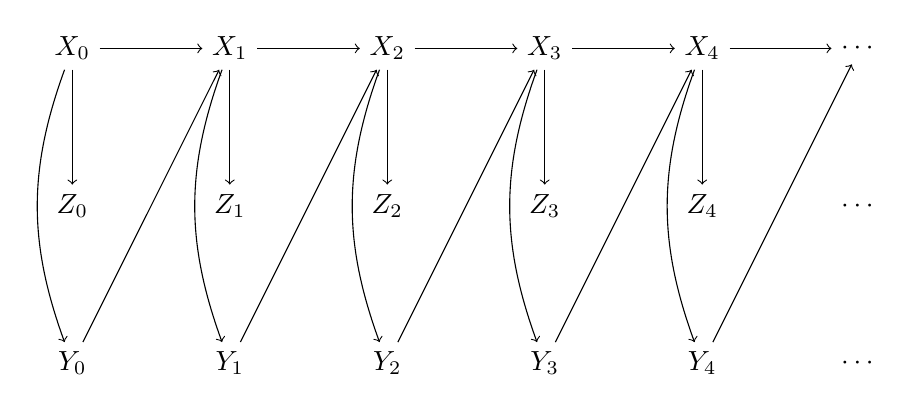
\begin{tikzpicture}[xscale=2,yscale=2]
  \node (x0) at (0,2){$X_0$};
  \node (x1) at (1,2){$X_1$};
  \node (x2) at (2,2){$X_2$};
  \node (x3) at (3,2){$X_3$};
  \node (x4) at (4,2){$X_4$};
  \node (x5) at (5,2){$\cdots$};

  \node (z0) at (0,1){$Z_0$};
  \node (z1) at (1,1){$Z_1$};
  \node (z2) at (2,1){$Z_2$};
  \node (z3) at (3,1){$Z_3$};
  \node (z4) at (4,1){$Z_4$};
  \node (z5) at (5,1){$\cdots$};

  \node (y0) at (0,0){$Y_0$};
  \node (y1) at (1,0){$Y_1$};
  \node (y2) at (2,0){$Y_2$};
  \node (y3) at (3,0){$Y_3$};
  \node (y4) at (4,0){$Y_4$};
  \node (y5) at (5,0){$\cdots$};

  \draw[->] (x0) -- (x1);
  \draw[->] (x1) -- (x2);
  \draw[->] (x2) -- (x3);
  \draw[->] (x3) -- (x4);
  \draw[->] (x4) -- (x5);

  \draw[->] (x0) -- (z0);
  \draw[->] (x1) -- (z1);
  \draw[->] (x2) -- (z2);
  \draw[->] (x3) -- (z3);
  \draw[->] (x4) -- (z4);

	\draw[->] (x0) to[bend right=20] (y0); 
	\draw[->] (x1) to[bend right=20] (y1); 
	\draw[->] (x2) to[bend right=20] (y2); 
	\draw[->] (x3) to[bend right=20] (y3); 
	\draw[->] (x4) to[bend right=20] (y4);
	
	\draw[->] (y0) -- (x1);
	\draw[->] (y1) -- (x2);
	\draw[->] (y2) -- (x3);
	\draw[->] (y3) -- (x4);
	\draw[->] (y4) -- (x5);

\end{tikzpicture}
\caption{The Inter-Dependencies of $X_t$,$Y_t$, and $Z_t$ for the Case as Described by Dragan }
\label{Ancdep}
\end{figure}

Let us consider the process determined by $X_t,Y_t$, and $Z_t$ which depend on each other as specified in Figure~\ref{Ancdep}. 
The major difference to our previous diagram in Figure~\ref{HMMdep} is that the actions are determined by the world-states directly instead of inferring them from a previous history of actions and observables. 

For our example of a game of Tic-Tac-Toe, this would correspond to us (the observer) watching the agent playing the game. The difference between the observer and the agent consists in that the agent has his/her glasses on and can perfectly observe the board state, while we are not able to do so. That is the agent can make decisions based on the real world-state. 
To model this, we use very similar tools to the previous times. We proceed as before except for how an action is chosen. 

We define $M^{a_j} \in \mathbb{R}^{n\times n}$ with 
\[
M^{a_j}_{x,y}:=P(X_{t+1}=q_x|X_t=q_y,Y_t=a_j)
\]
This is again essentially the same $M^{a_j}$ we have used for the previous situations.
Then we define a matrix $P\in \mathbb{R}^{n\times m}$ with 
\[
P_{j,i}:=P(Y_t=a_j|X_t=q_i)=P(Y_t=a_j|X_t=q_i,h)
\]
In contrast to our previous definition of $P$ in Section \ref{sec:HMM} we now have an explicit probabilistic interpretation of the entries of $P$. 
We collect observation probabilities in a diagonal matrix $O_{o_e}$ with 
\[
(O_{o_e})_{i,i}=P(Z_t=o_e|X_t=q_i)=P(Z_t=o_e|X_t=q_i,Y_t=a_j)
\]
Then as before we define $w_t \in \mathbb{R}^{n}$ with 
\[
w_t:=
\left ( 
\begin{matrix}
P(X_t=q_1|h) \\
P(X_t=q_2|h) \\
\vdots \\
P(X_t=q_n|h)
\end{matrix}
\right )
\]
Here we see a fundamental difference in the knowledge of the observer and the agent. From the agent's perspective, this is $e_i$, depending on the world-state he sees. From the observers perspective this can a priori be any element of $\mathbb{R}^{n} $ with non-negative entries summing to $1$. We always use the observer perspective though. If we were to use the agent perspective, there is no difference to the MC case anymore.

To predict the future we again define a vector $w_t^{t+k} \in \mathbb{R}^{n}$ 
\[
w_t^{t+k}:=
\left ( 
\begin{matrix}
P(X_{t+k}=q_1|h) \\
P(X_{t+k}=q_2|h) \\
\vdots \\
P(X_{t+k}=q_n|h)
\end{matrix}
\right )
\]
In this new process, the action the agent chooses can tell us a lot about the world-states. For instance, if the agent only took $a_1$ if the world was in state $q_1$, then if we see the agent take $a_1$, the world must have been in world-state $q_1$.  
To represent this we define diagonal matrices $O_{a_j}$ by
\[
(O_{a_j})_{i,i}:=P(Y_t=a_j|X_t=q_i)=P_{j,i}
\]
This corresponds to us essentially treating the actions as an observable. 

To combine these two observation matrices we define $O_{a_j,o_e}=O_{a_j}*O_{o_e}$. 
\begin{prop} 
$(O_{a_j,o_e})_{i,i}=P(Y_t=a_j,Z_t=o_e|X_t=q_i)$
\end{prop}
\begin{proof}
\begin{align*}
(O_{a_j,o_e})_{i,i}&=(O_{a_j})_{i,i}\cdot (O_{o_e})_{i,i} \\
&=P(Y_t=a_j|X_t=q_i)\cdot P(Z_t=o_e|X_t=q_i) \\
&=P(Y_t=a_j,Z_t=o_e|X_t=q_i)
\end{align*}
\end{proof}
Then we define $T^{a_j}_{o_e}=M^{a_j}*O_{a_j,o_e}$. Note that this is not the same as the notion of operators from OOMs, as $M^{a_j}$ is not equal to the sum of $T^{a_j}_{o_e}$ over $o_e$.
\begin{prop}
$(T^{a_j}_{o_e})_{x,y}=P(X_{t+1}=q_x,Z_t=o_e,Y_{t}=a_j|X_t=q_y)$
\end{prop}
\begin{proof}
\begin{align*}
(T^{a_j}_{o_e})_{x,y}&=M^{a_j}_{x,y}\cdot (O_{o_e,a_j})_{y,y} \\
&=P(X_{t+1}=q_x|Y_t=a_j,X_{t}=q_y)\cdot P(Y_t=a_j,Z_t=o_e|X_{t}=q_y) \\
&=P(X_{t+1}=q_x,Z_t=o_e,Y_{t}=a_j|X_t=q_y)
\end{align*}
\end{proof}
Then we can use this to get a straightforward update equation. 
\begin{prop}
$P(X_{t+1}=q_i|Y_t=a_j,Z_t=o_e,h)=\frac{T^{a_j}_{o_e}w_t}{\vec{1} T^{a_j}_{o_e}w_t}[i]$
\end{prop}
\begin{proof}
\begin{align*}
\frac{T^{a_j}_{o_e}w_t}{\vec{1} T^{a_j}_{o_e}w_t}[i]&=\frac{(T^{a_j}_{o_e}w_t)[i]}{\vec{1} T^{a_j}_{o_e}w_t} \\
&=\frac{\sum\limits_{d=1}^{n} (T^{a_j}_{o_e})_{i,d}\cdot w_t[d]}{\sum\limits_{i=1}^{n} \sum\limits_{d=1}^{n} (T^{a_j}_{o_e})_{i,d}\cdot w_t[d]} \\
&=\frac{\sum\limits_{d=1}^{n} P(X_{t+1}=q_i,Z_t=o_e,Y_{t}=a_j|X_t=q_d) P(X_t=q_d|h)}{\sum\limits_{i=1}^{n}\sum\limits_{d=1}^{n} P(X_{t+1}=q_i,Z_t=o_e,Y_{t}=a_j|X_t=q_d) P(X_t=q_d|h)} \\
&=\frac{\sum\limits_{d=1}^{n} P(X_{t+1}=q_i,Z_t=o_e,Y_{t}=a_j|X_t=q_d,h) P(X_t=q_d|h)}{\sum\limits_{i=1}^{n}\sum\limits_{d=1}^{n} P(X_{t+1}=q_i,Z_t=o_e,Y_{t}=a_j|X_t=q_d,h) P(X_t=q_d|h)} \\
&=\frac{\sum\limits_{d=1}^{n} P(X_{t+1}=q_i,Z_t=o_e,Y_t=a_j,X_t=q_d|h)}{\sum\limits_{i=1}^n \sum\limits_{d=1}^{n} P(X_{t+1}=q_i,Z_t=o_e,Y_t=a_j,X_t=q_d|h) } \\
&=\frac{P(X_{t+1}=q_i,Z_t=o_e,Y_t=a_j|h)}{P(Z_t=o_e,Y_t=a_j|h)} \\
&=P(X_{t+1}=q_i|Y_t=a_j,Z_t=o_e,h)
\end{align*}
\end{proof}
Now we look at predicting the future.
We first look at what $T^{a_j}_{o_e}*w_t^{t+k}$ is. 
\begin{prop}
$T^{a_j}_{o_e}*w_t^{t+k}=P(X_{t+k+1}=q_i,X_{t+k}=o_e,Y_{t+k}=a_j|h)$
\end{prop}
\begin{proof}
\begin{align*}
((T^{a_j}_{o_e})*w_t^{t+k})[i]&=\sum\limits_{d=1}^{n} (T^{a_j}_{o_e})_{i,d}*w_t^{t+k}[d] \\
&=\sum\limits_{d=1}^n P(X_{t+k+1}=q_i,Z_{t+k}=o_e,Y_{t+k}=a_j|X_{t+k}=q_d)\cdot P(X_{t+k}=q_d|h) \\
&=\sum\limits_{d=1}^n P(X_{t+k+1}=q_i,Z_{t+k}=o_e,Y_{t+k}=a_j|X_{t+k}=q_d,h)\cdot P(X_{t+k}=q_d|h) \\
&=\sum\limits_{d=1}^{n} P(X_{t+k+1}=q_i,X_{t+k}=o_e,Y_{t+k}=a_j,X_{t+k}=q_d|h) \\
&=P(X_{t+k+1}=q_i,X_{t+k}=o_e,Y_{t+k}=a_j|h)
\end{align*}
\end{proof}
Using this result, we can now look at how to compute the future using this model. 
\begin{prop}
$w_t^{t+k}[i]=\sum\limits_{e=1}^{K} \sum\limits_{j=1}^{m} (T^{a_j}_{o_e}*w_t^{t+k})[i]$
\end{prop}
\begin{proof}
\begin{align*}
w_t^{t+k}[i]&=P(X_{t+k+1}=q_i|h) \\
&=\sum\limits_{e=1}^{K} \sum\limits_{j=1}^{m} P(X_{t+k+1}=q_i,Y_{t+k}=a_j,Z_{t+k}=o_e|h) \\
&=\sum\limits_{e=1}^{K} \sum\limits_{j=1}^{m} (T^{a_j}_{o_e}*w_t^{t+k})[i]
\end{align*}
\end{proof}
Therefore we have found a nice iterative way to compute $w_t^{t+k}$, which makes computation of $w_t^{t+k}$ take linear time in $k$.

Now that we have a cheap way to predict the future, we just need to find a way to represent this process using  a HMM with observables from $O\times A$. The resulting HMM will consist of the Markov matrix and observation matrices as in Section \ref{sec:HMM}, except that there is no need for $\Phi$ anymore.
As indicated, we define $M$ as before with $M_{(i_1-1)\cdot m+j_1,(i_2-1)\cdot m+j_2}=M^{a_{j_2}}_{i_1,i_2}\cdot P_{j_1,i_1}$. 

\begin{prop}
$M_{(i_1-1)\cdot m+j_1,(i_2-1)\cdot m+j_2}=P(Y_{t+1}=a_{j_1},X_{t+1}=q_{i_1}|Y_t=a_{j_2},X_t={q_{i_2}})$ 
\end{prop}
\begin{proof}
\begin{align*}
M_{(i_1-1)\cdot m+j_1,(i_2-1)\cdot m+j_2}=&M^{a_{j_2}}_{i_1,i_2}\cdot P_{j_1,i_1} \\
=&P(X_{t+1}=q_{i_1}|Y_t=a_{j_2},X_t=q_{i_2})\cdot P(Y_{t+1}=a_{j_1}|X_{t+1}=q_{i_1}) \\
=&P(X_{t+1}=q_{i_1}|Y_t=a_{j_2},X_t=q_{i_2})\\
 &  \cdot P(Y_{t+1}=a_{j_1}|X_{t+1}=q_{i_1},Y_t=a_{j_2},X_t=q_{i_2}) \\
=&P(X_{t+1}=q_{i_1},Y_{t+1}=a_{j_1}|Y_t=a_{j_2},X_t=q_{i_2})
\end{align*}
\end{proof}
Now we again define $O_{o_e,a_j}$, with entries $(O_{o_e,a_{j_1}})_{(i-1)\cdot m+j,(i-1)\cdot m+j}=\delta_{j,j_1}(O_{o_e})_{i,i}$ and $T_{a_j,o_e}=M*O_{o_e,a_j}$. 
\begin{prop}
$(T_{a_j,o_e}){(i_1-1)\cdot m+ j_1,(i_2-1)\cdot m+j_2}=P(Y_{t+1}=a_{j_1},X_{t+1}=q_{i_1},Z_t=o_e,Y_t=a_j|X_t=q_{i_2},Y_t=a_{j_2})$
\end{prop}
\begin{proof}
\begin{align*}
&(T_{a_j,o_e}){(i_1-1)\cdot m+ j_1,(i_2-1)\cdot m+j_2}\\
=&\sum\limits_{d_1=1}^{n} \sum\limits_{d_2=1}^m M_{(i_1-1)\cdot m+j_1,(d_1-1)\cdot m+d_2} \cdot (O_{o_e,a_j})_{(d_1-1)\cdot m+d_2,(i_2-1)\cdot m+j_2} \\
=&M_{(i_1-1)\cdot m+j_1,(i_2-1)\cdot m+j_2} \cdot (O_{o_e,a_j})_{(i_2-1)\cdot m+j_2,(i_2-1)\cdot m+j_2} \\
=&P(X_{t+1}=q_{i_1},Y_{t+1}=a_{j_1}|Y_t=a_{j_2},X_t=q_{i_2})\cdot (\delta_{j,j_2} (O_{o_e})_{i_2,i_2}) \\
=&P(X_{t+1}=q_{i_1},Y_{t+1}=a_{j_1}|Y_t=a_{j_2},X_t=q_{i_2})\cdot (\delta_{j,j_2} P(Z_t=o_e|X_{t}=q_{i_2},Y_{t}=a_{j_2})) \\
=&P(X_{t+1}=q_{i_1},Y_{t+1}=a_{j_1}|Y_t=a_{j_2},X_t=q_{i_2})\cdot P(Z_t=o_e|X_{t}=q_{i_2},Y_{t}=a_{j_2}) \cdot \delta_{j,j_2} \\
=&P(X_{t+1}=q_{i_1},Y_{t+1}=a_{j_1},Z_t=o_e|Y_t=a_{j_2},X_t=q_{i_2})\cdot \delta_{j,j_2} \\
=&P(X_{t+1}=q_{i_1},Y_{t+1}=a_{j_1},Z_t=o_e,Y_t=a_j|Y_t=a_{j_2},X_t=q_{i_2})
\end{align*}
\end{proof}
As claimed before, we get the update equation without the need for $\Phi$. 
\begin{prop}
$P(X_{t+1}=q_i,Y_{t+1}=a_j|Z_t=o_e,Y_t=a_{j_1},h)=\frac{T_{a_{j_1},o_e}*\widetilde{w_t}}{\vec{1}*T_{a_{j_1},o_e}*\widetilde{w_t}}[(i-1)\cdot m+j]$ 
\end{prop}
\begin{proof}
\begin{align*}
&\frac{T_{a_{j_1},o_e}*\widetilde{w_t}}{\vec{1}*T_{a_{j_1},o_e}*\widetilde{w_t}}[(i-1)\cdot
  m+j]j\\
=&\frac{\sum\limits_{d_1=1}^{n} \sum\limits_{d_2=1}^m (T_{a_{j_1},o_e})_{(i-1)\cdot m+j,(d_1-1)\cdot m+d_2}\cdot w_t[(d_1-1)\cdot m+ d_2]}{\sum\limits_{i=1}^n \sum\limits_{j=1}^m \sum\limits_{d_1=1}^{n} \sum\limits_{d_2=1}^m (T_{a_{j_1},o_e})_{(i-1)\cdot m+j,(d_1-1)\cdot m+d_2}\cdot w_t[(d_1-1)\cdot m+ d_2]} \\
=&\frac{\sum\limits_{d_1=1}^{n} \sum\limits_{d_2=1}^m P(Y_t=a_{j_1},Y_{t+1}=a_j,X_{t+1}=q_i,Z_t=o_e|X_t=q_{d_1},Y_t=a_{d_2}) \cdot P(X_t=q_{d_1},Y_t=a_{d_2}|h)}{\sum\limits_{i=1}^n \sum\limits_{j=1}^m\sum\limits_{d_1=1}^{n} \sum\limits_{d_2=1}^m P(Y_t=a_{j_1},Y_{t+1}=a_j,X_{t+1}=q_i,Z_t=o_e|X_t=q_{d_1},Y_t=a_{d_2}) \cdot P(X_t=q_{d_1},Y_t=a_{d_2}|h)} \\
=&\frac{\sum\limits_{d_1=1}^n \sum\limits_{d_2=1}^m P(Y_t=a_{j_1},Y_{t+1}=a_j,X_{t+1}=q_i,X_t=q_{d_1},Y_t=a_{d_2},Z_t=o_e|h) }{\sum\limits_{i=1}^n \sum\limits_{j=1}^m \sum\limits_{d_1=1}^n \sum\limits_{d_2=1}^m P(Y_t=a_{j_1},Y_{t+1}=a_j,X_{t+1}=q_i,X_t=q_{d_1},Y_t=a_{d_2},Z_t=o_e|h)} \\
=&\frac{P(Y_{t+1}=a_j,Y_t=a_{j_1},X_{t+1}=q_i,Z_t=o_e|h)}{\sum\limits_{i=1}^{n} \sum\limits_{j=1}^m P(Y_{t+1}=a_j,Y_t=a_{j_1},X_{t+1}=q_i,Z_t=o_e|h)}\\ 
=&\frac{P(Y_{t+1}=a_j,Y_t=a_{j_1},X_{t+1}=q_i,Z_t=o_e|h)}{P(Z_t=o_e,Y_t=a_{j_1}|h)} \\ 
=& P(Y_{t+1}=a_j,X_{t+1}=q_i|Y_t=a_{j_1},Z_t=o_e,h)
\end{align*}
\end{proof}
As we can see this is a valid HMM. Therefore we can use the standard method for predicting future HMM probability distributions. 
\begin{prop}
\[P(X_{t+k+1}=q_i,Y_{t+k+1}=a_j|h)=(M*w_{t}^{t+k})[(i-1)\cdot m+j]\]
\end{prop}
\begin{proof}
\begin{align*}
&(M*w_{t}^{t+k})[(i-1)\cdot m+j]\\
=&\sum\limits_{d_1=1}^n \sum\limits_{d_2=1}^m M_{(i-1)\cdot m+j,(d_1-1)\cdot m+d_2|} \cdot w_t^{t+k}[(d_1-1)\cdot m+d_2]  \\
=&\sum\limits_{d_1=1}^n \sum\limits_{d_2=1}^m P(X_{t+k+1}=q_i,Y_{t+k+1}=a_j|X_{t+k}=q_{d_1},Y_{t+k}=q_{d_2})\cdot P(X_{t+k}=q_{d_1},Y_{t+k}=a_{d_2}|h) \\
=&\sum\limits_{d_1=1}^n \sum\limits_{d_2=1}^m P(X_{t+k+1}=q_i,Y_{t+k+1}=a_j|X_{t+k}=q_{d_1},Y_{t+k}=q_{d_2},h)\cdot P(X_{t+k}=q_{d_1},Y_{t+k}=a_{d_2}|h) \\
=&\sum\limits_{d_1=1}^n \sum\limits_{d_2=1}^m P(X_{t+k+1}=q_i,Y_{t+k+1}=a_j,X_{t+k}=q_{d_1},Y_{t+k}=q_{d_2}|h) \\
=&P(X_{t+k+1}=q_i,Y_{t+k+1}=a_j|h) \\
=&w_t^{t+k+1}[(i-1)\cdot m+j]
\end{align*}
\end{proof}
Hence we have shown that this process, where we are essentially watching an agent decide on the basis of a MDP, can be represented by a normal HMM, and we can even predict the future cheaply. However, this process and the predictions are not well suited to planning, as for planning tasks the observer needs to decide on actions, not the agent itself. Normally there is no distinction made, but here we need to, since the agent has access to more information than the observer. 

As a consequence we know that a subset of HMMs, that is, that subset where these definitions would make sense, with observables $O\times A$ model a process that is not well suited for planning. Thus, we can also conjecture that it is not possible to model POMDPs with a policy using  a HMM with observables $O\times A$.
\section{Conclusion}\label{sec:conc}
This thesis develops a theoretical foundation for Dragan's embedded policy approach. Based on this we have investigated whether Dragan's algorithm can be improved by substituting MDPs/POM\-DPs/IO-OOMs with a policy for the OOM that Dragan uses in her algorithm. 

We have fulfilled the first of three goals from Section \ref{sec:Dragan}. However, we found out that it was not possible to achieve the second goal in general and thus it is not possible to satisfy the third goal in the general case. 

We have found a way to use the embedded policy approach using a MDP and a policy, by modeling MDPs with a policy by MCs with world-states $Q\times A$. We furthermore constructed MCs with world-states $Q$, that model the same MDP and policy, which allow for cheaper prediction of the future. Therefore, we have fulfilled the MC goal, as we now know the theoretical background for this special case. 

Unfortunately, we have been unable to find a way to use the EPA with a POMDP and a policy, except in the special case where actions and world-states are independent, as computing the probability of future states is prohibitively expensive. Hence the HMM goal still defies our efforts and may even be unachievable.  

Nevertheless, we have been able to prove that at least a subset of HMMs with observables $O\times A$, that is, a subset of matrices with embedded policies, model a very POMDP-like process; it only differs from a POMDP in that while the observe still cannot see the world-state, the agent can. However, this process is not well suited for planning, since in planning algorithms the observer needs to make decisions and does not have the same information. Although we have found a way to use the embedded policy approach for these processes, it is not possible to design an algorithm to make use of it. We thus conclude that, while we were not able to fulfill the HMM goal, Dragan's algorithm wasn't able to either, as she was modeling these unsuitable processes and not POMDPs. 

Finally, we did no work on fulfilling the OOM goal, as the previous result casts a strong doubt on whether it is even desirable to fulfill it, since possibly only processes are modeled that cannot be used for planning.

An interesting avenue of research might be trying to model POMDPs using MDPs, as we have shown that the embedded policy approach works for MDPs. Additionally it might be interesting to test whether Dragan's algorithm works for OOMs, as while we have shown that it does not work in the general case, there might be enough special cases that it is still a useful algorithm.

\paragraph{Acknowledgments}
I would first like to thank Prof. Jaeger for his tremendous help in the creation of this
thesis. In his course I first discovered my interest in Machine Learning. I would
additionally like to thank him for his patience in dealing with my numerous forays into
speculation and always making me come back and rigorously define my ideas. Finally he
helped keep me on course when I was panicking and thought I couldn't finish my thesis.
Additionally I would like to thank Dr. Mallahi Karai for being available as a mathematical
co-supervisor.

\bibliographystyle{alpha}
\bibliography{GR}
\end{document}
%%% Local Variables:
%%% mode: latex
%%% TeX-master: t
%%% End:

%  LocalWords:  flushright includegraphics bsc-logo vspace textbf mytitle myname vfill th
%  LocalWords:  mysupervisor hline flushleft textwidth newpage noindent emph Bellmann ako
%  LocalWords:  tableofcontents 4curr Kae4 Qlearn ednote koenntest MDPcomplex MCs bigskip
%  LocalWords:  conc summarized ldots mathbb vec geq cdot mathcal mcgoal hmmgoal oomgoal
%  LocalWords:  rightarrow centering tikzpicture xscale yscale cdots Mardep visualized
%  LocalWords:  realization vdots setlength arraycolsep HMMdep qquad forall normalizing
%  LocalWords:  probSeq normalized faende zusaetzlich referenzieren waere unabhaengig
%  LocalWords:  erwaehnst Kronecker-delta compactitem Ancdep Mallahi Karai
